\section{Problem Set 4}

\subsection{These are Relative Orbits}

\subsubsection{Initial Conditions}
For the first part of this problem, we set the initial conditions in classical orbital elements to be [6780000, 0.001, 0, 0, 0, 0]. This provides us with an eccentric orbit that is sufficiently far from the attractor's center. We then set the deputy's rtn coordinates to be [-50; -500; -180; -0.4; 0.1; 0], as we did in the last pset.

As requested for the second part, we keep the same initial orbit, but we set the osculating quasi non singular orbital elements to be [0, 100, 50, 100, 30, 200].

\subsubsection{Orbital Elements, Relative Orbital Elements}
First part, without J2:
\begin{figure}[H]
    \centering
    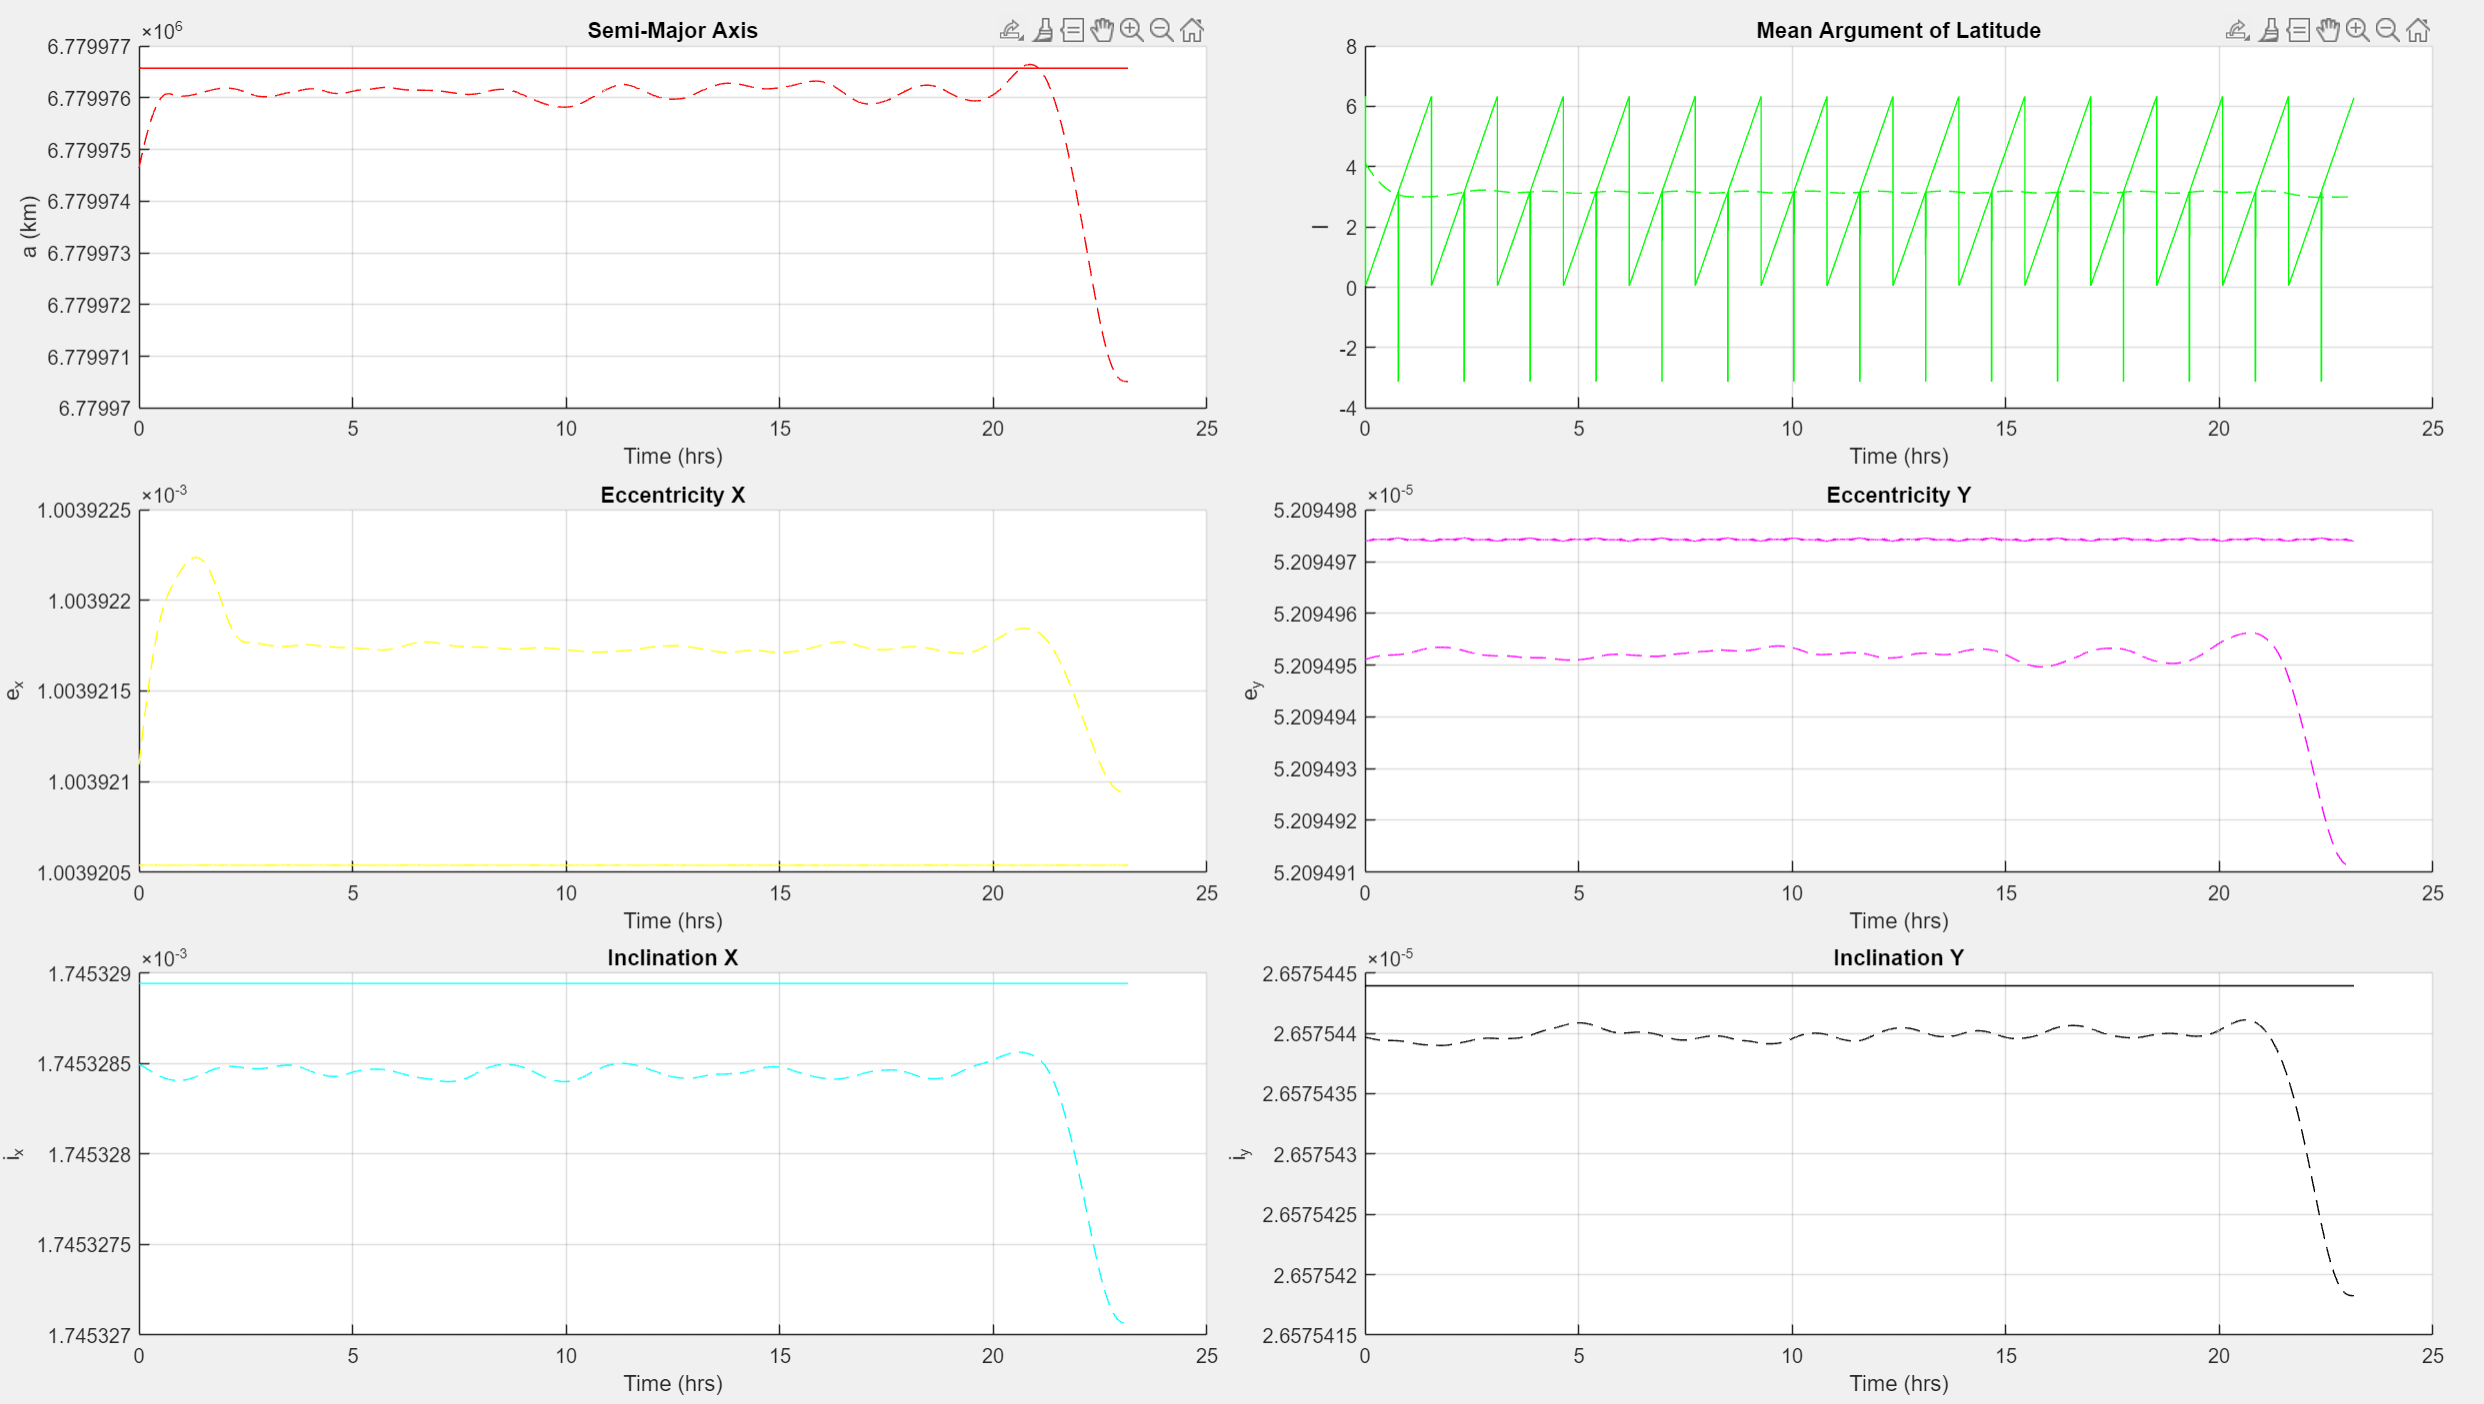
\includegraphics[width=0.7\textwidth]{PS4/Figures/case1_noJ2.png}
    \caption{Initial Conditions 1, Without J2, Quasi Nonsingular Orbital Elements}
    \label{fig:hcw_velocity}
\end{figure}
\begin{figure}[H]
    \centering
    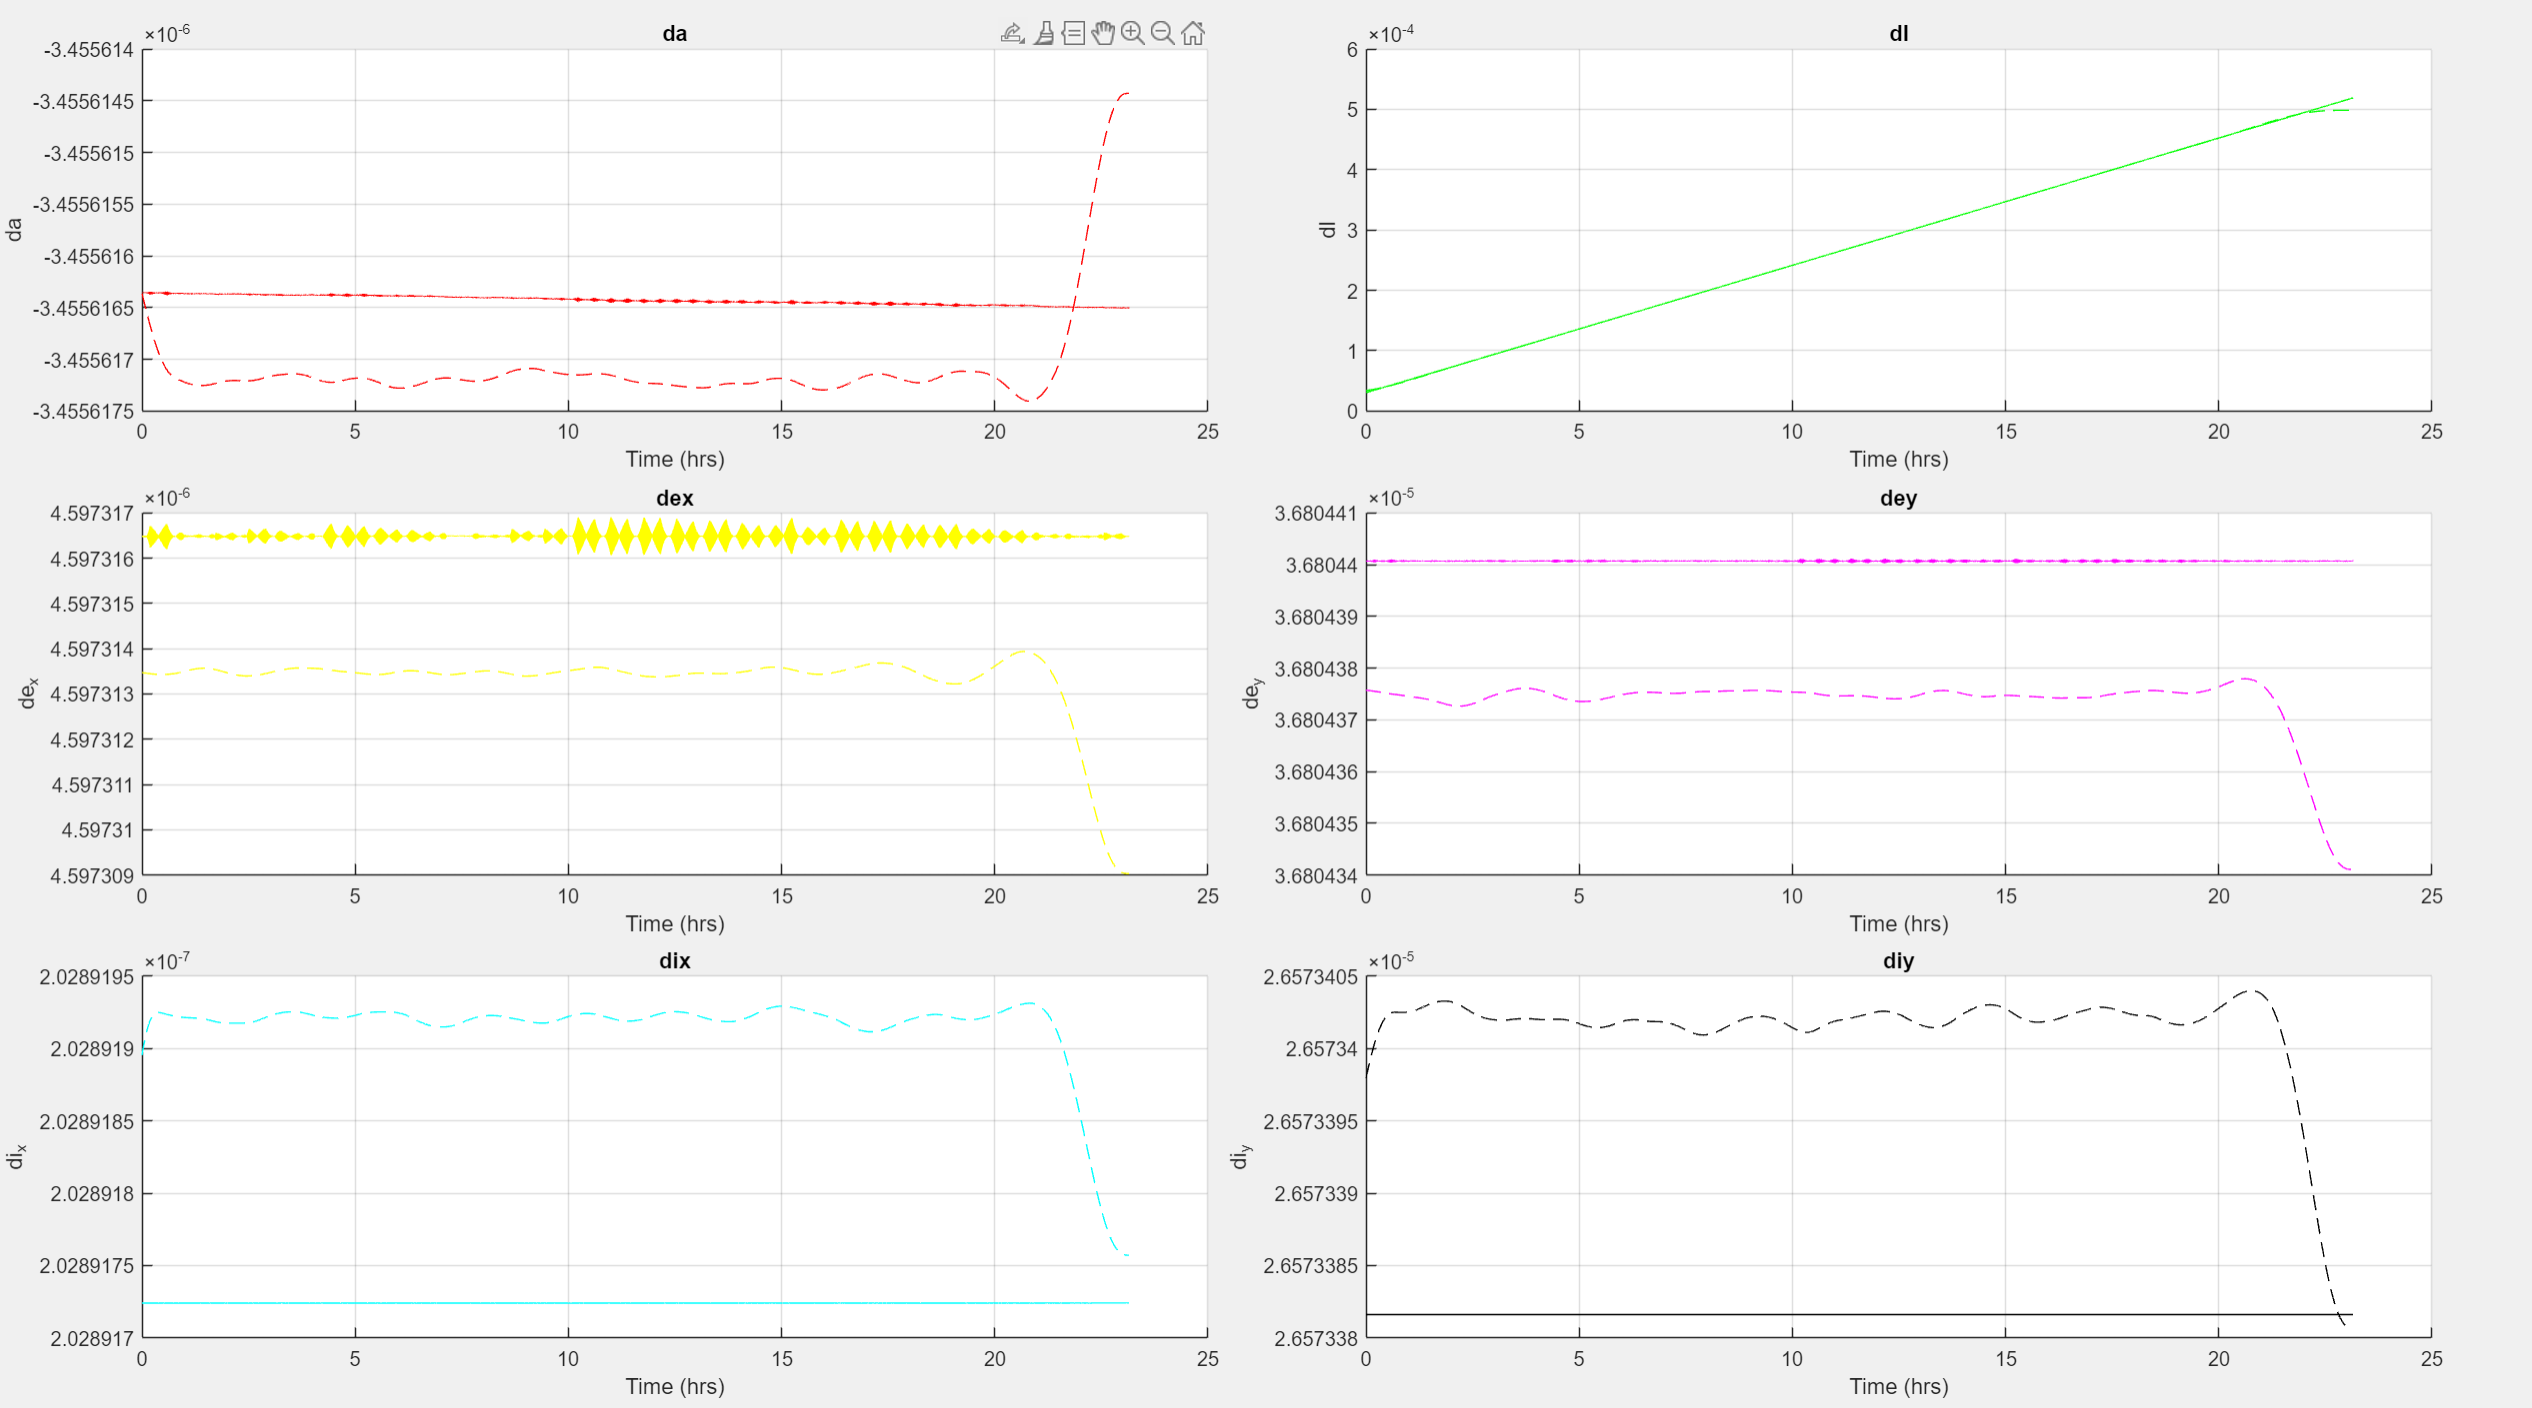
\includegraphics[width=0.7\textwidth]{PS4/Figures/case1_noJ2_2.png}
    \caption{Initial Conditions 1, Without J2, Quasi Nonsingular Relative Orbital Elements}
    \label{fig:hcw_velocity}
\end{figure}

First part, with J2:
\begin{figure}[H]
    \centering
    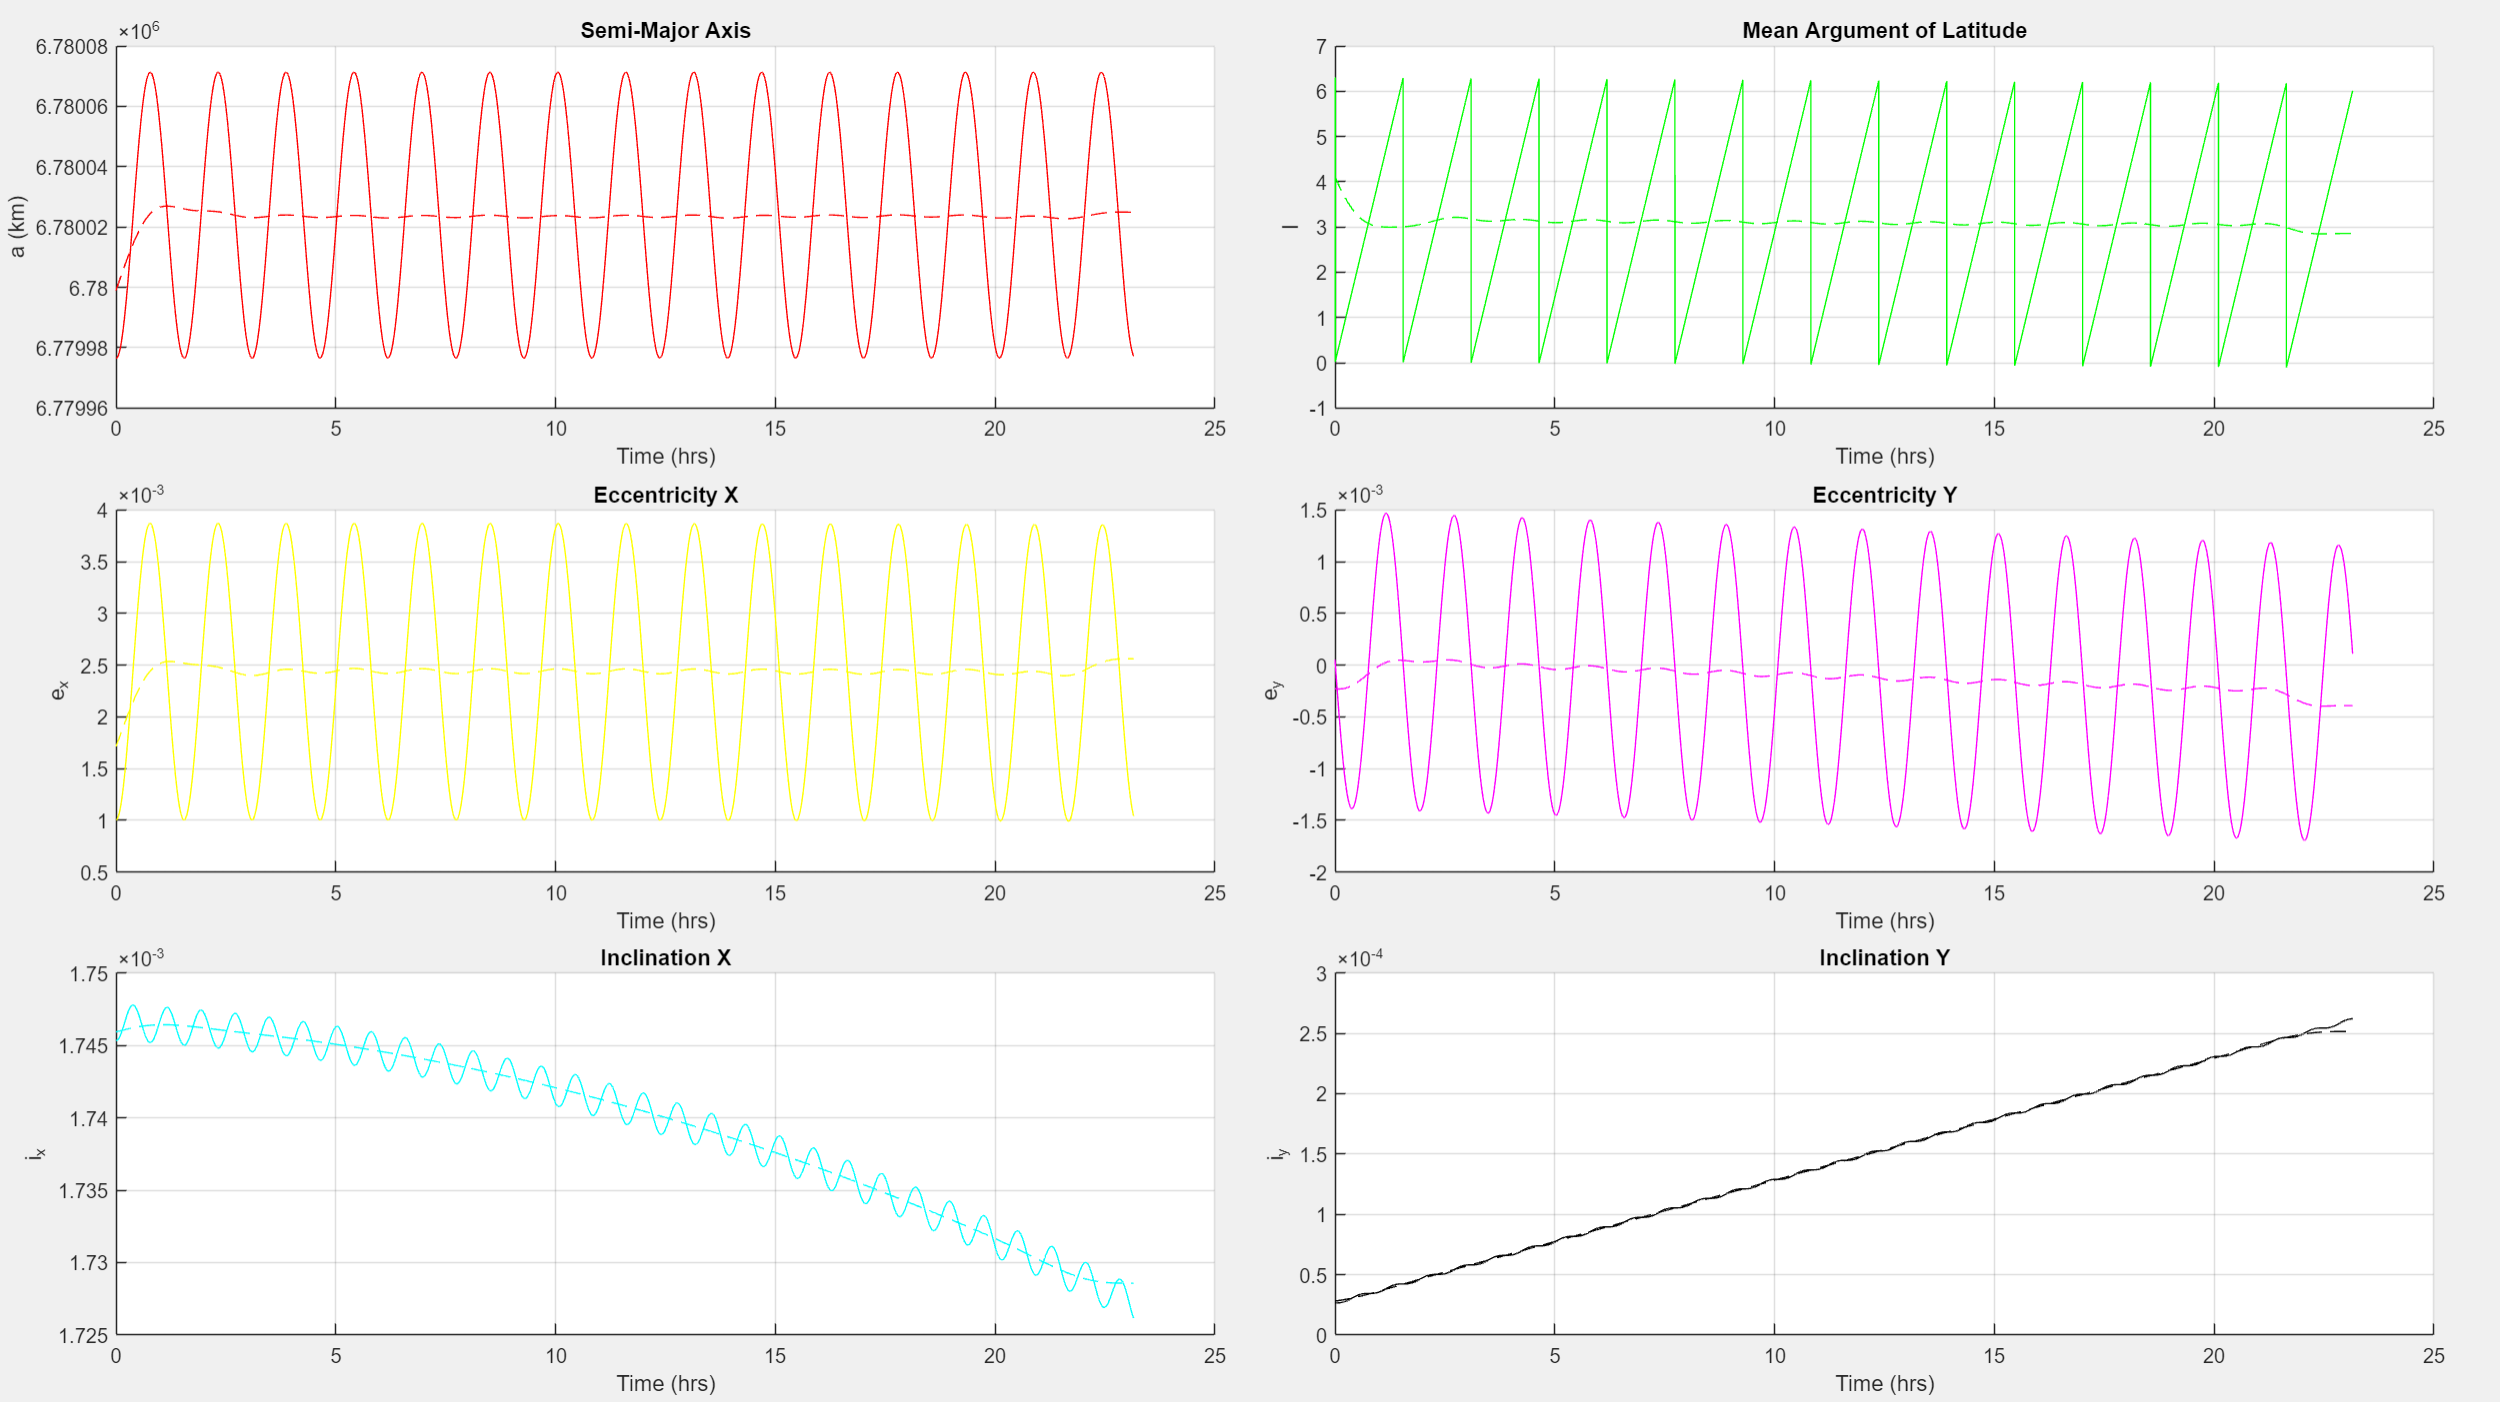
\includegraphics[width=0.7\textwidth]{PS4/Figures/case1_J2.png}
    \caption{Initial Conditions 1, With J2, Quasi Nonsingular Orbital Elements}
    \label{fig:hcw_velocity}
\end{figure}
\begin{figure}[H]
    \centering
    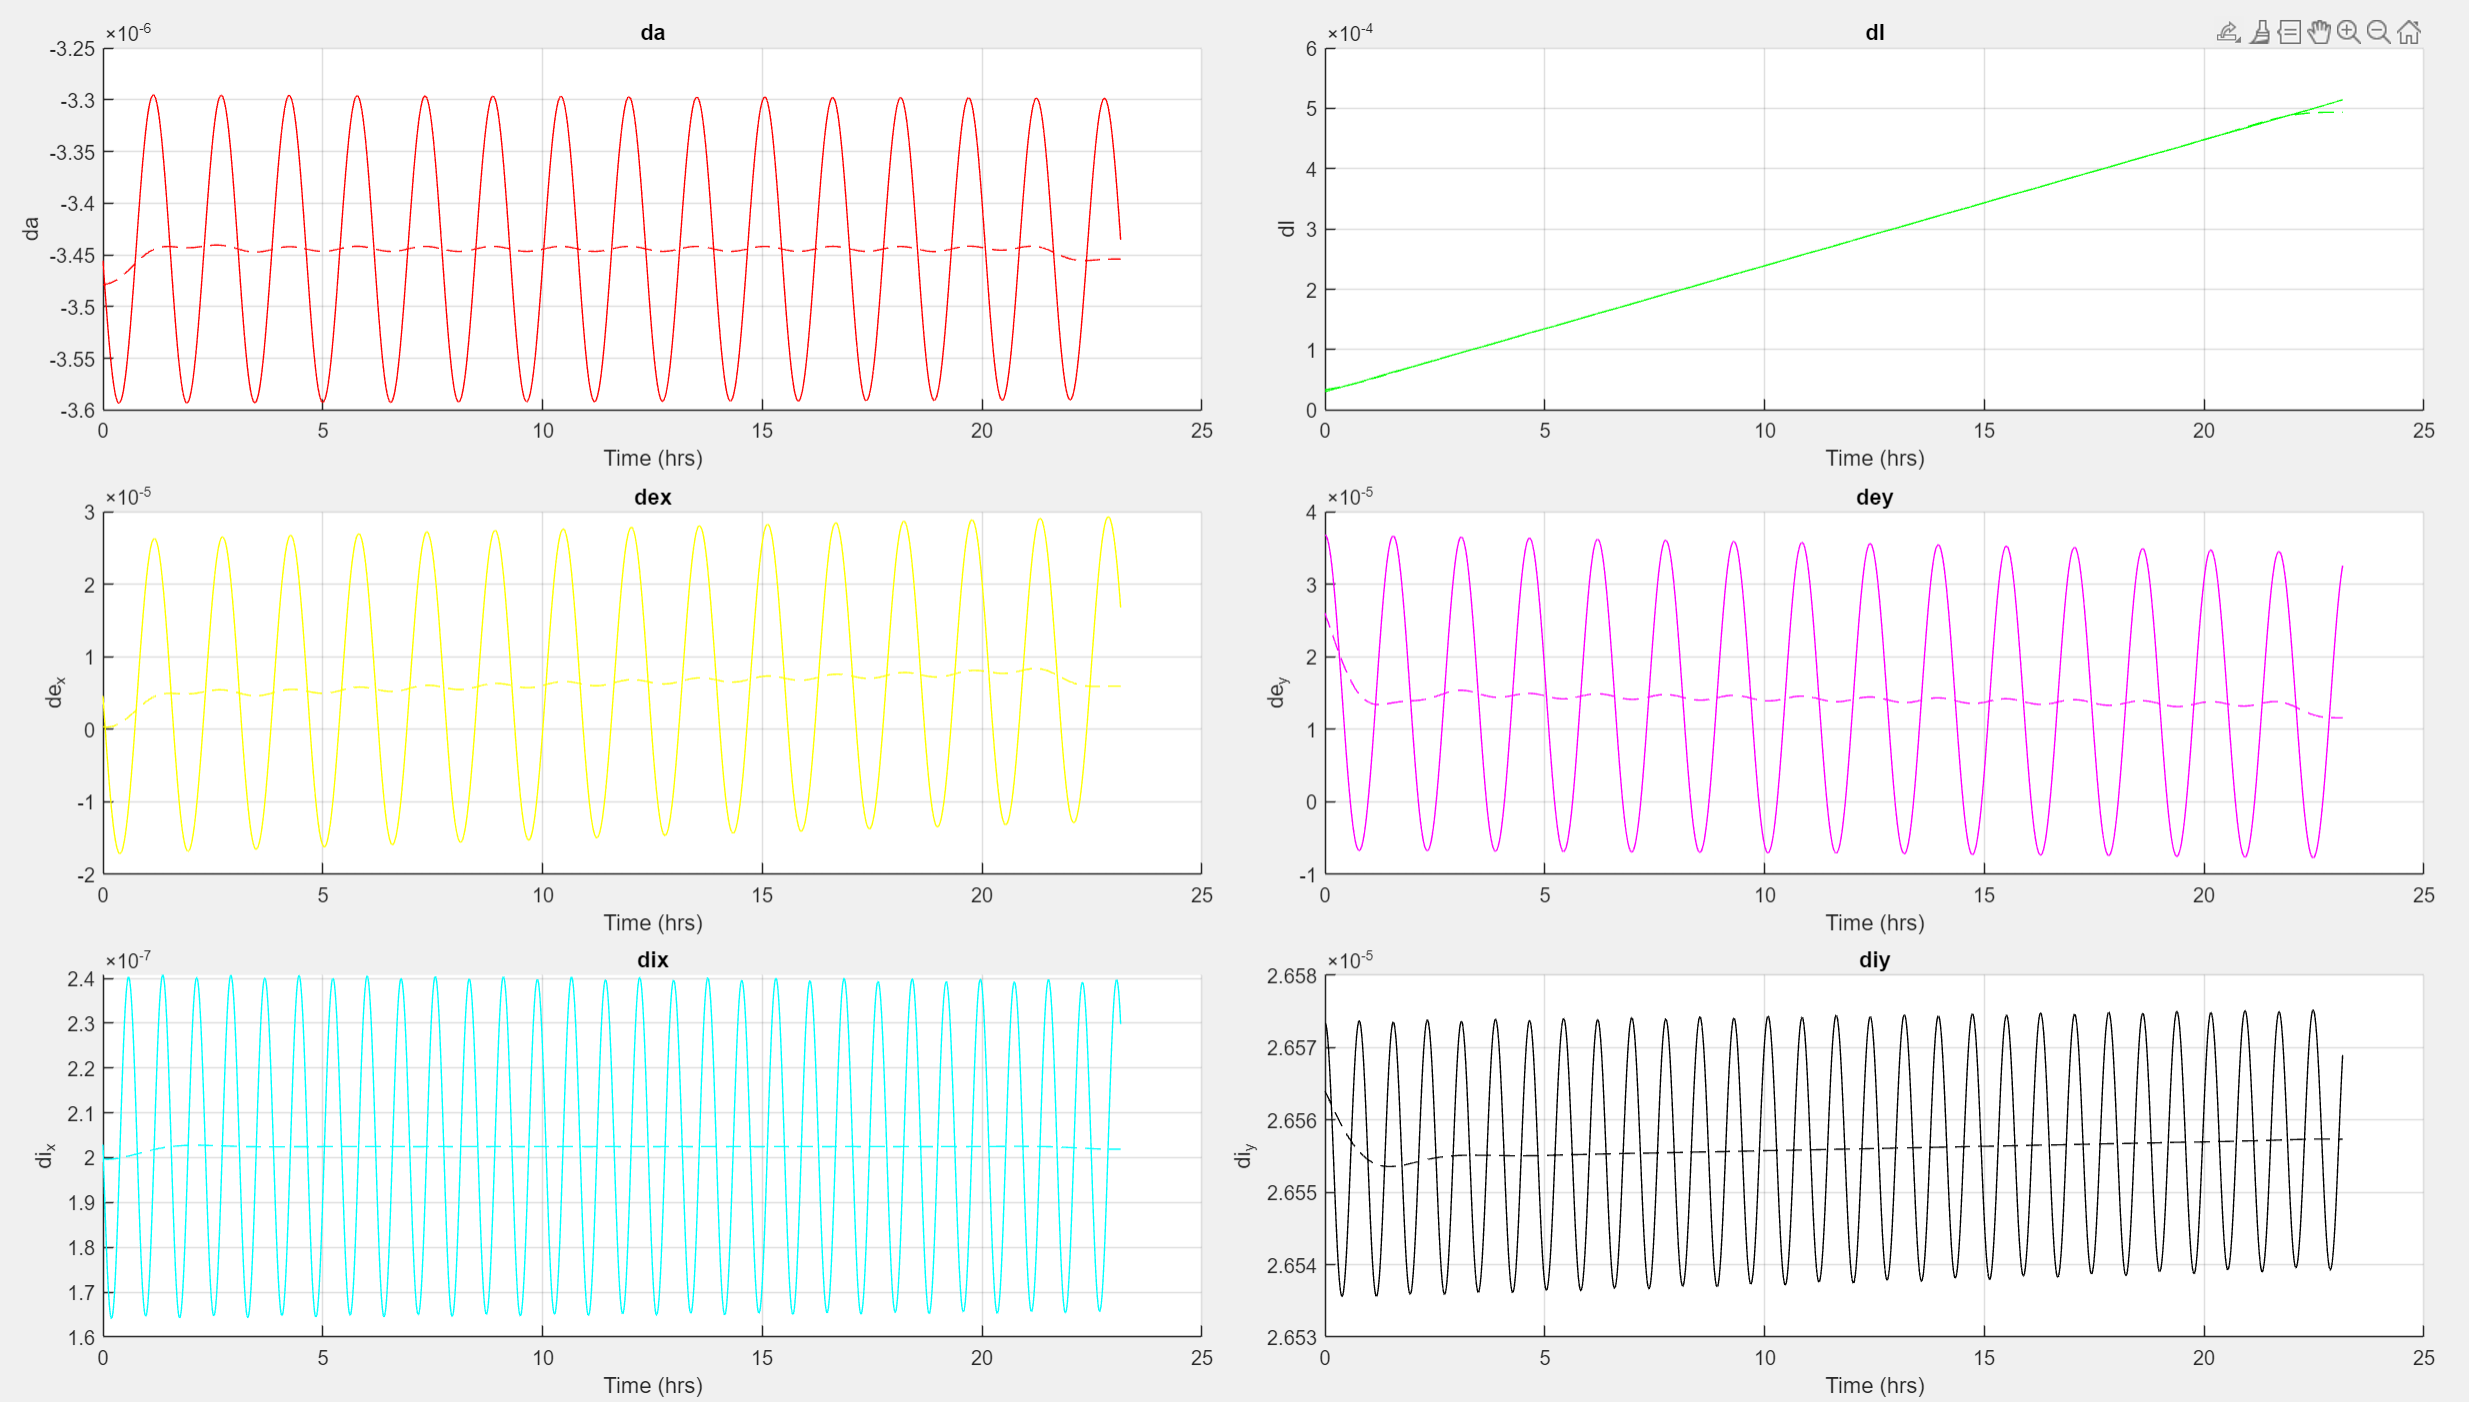
\includegraphics[width=0.7\textwidth]{PS4/Figures/case1_J2_2.png}
    \caption{Initial Conditions 1, With J2, Quasi Nonsingular Relative Orbital Elements}
    \label{fig:hcw_velocity}
\end{figure}
Second part, without J2:
\begin{figure}[H]
    \centering
    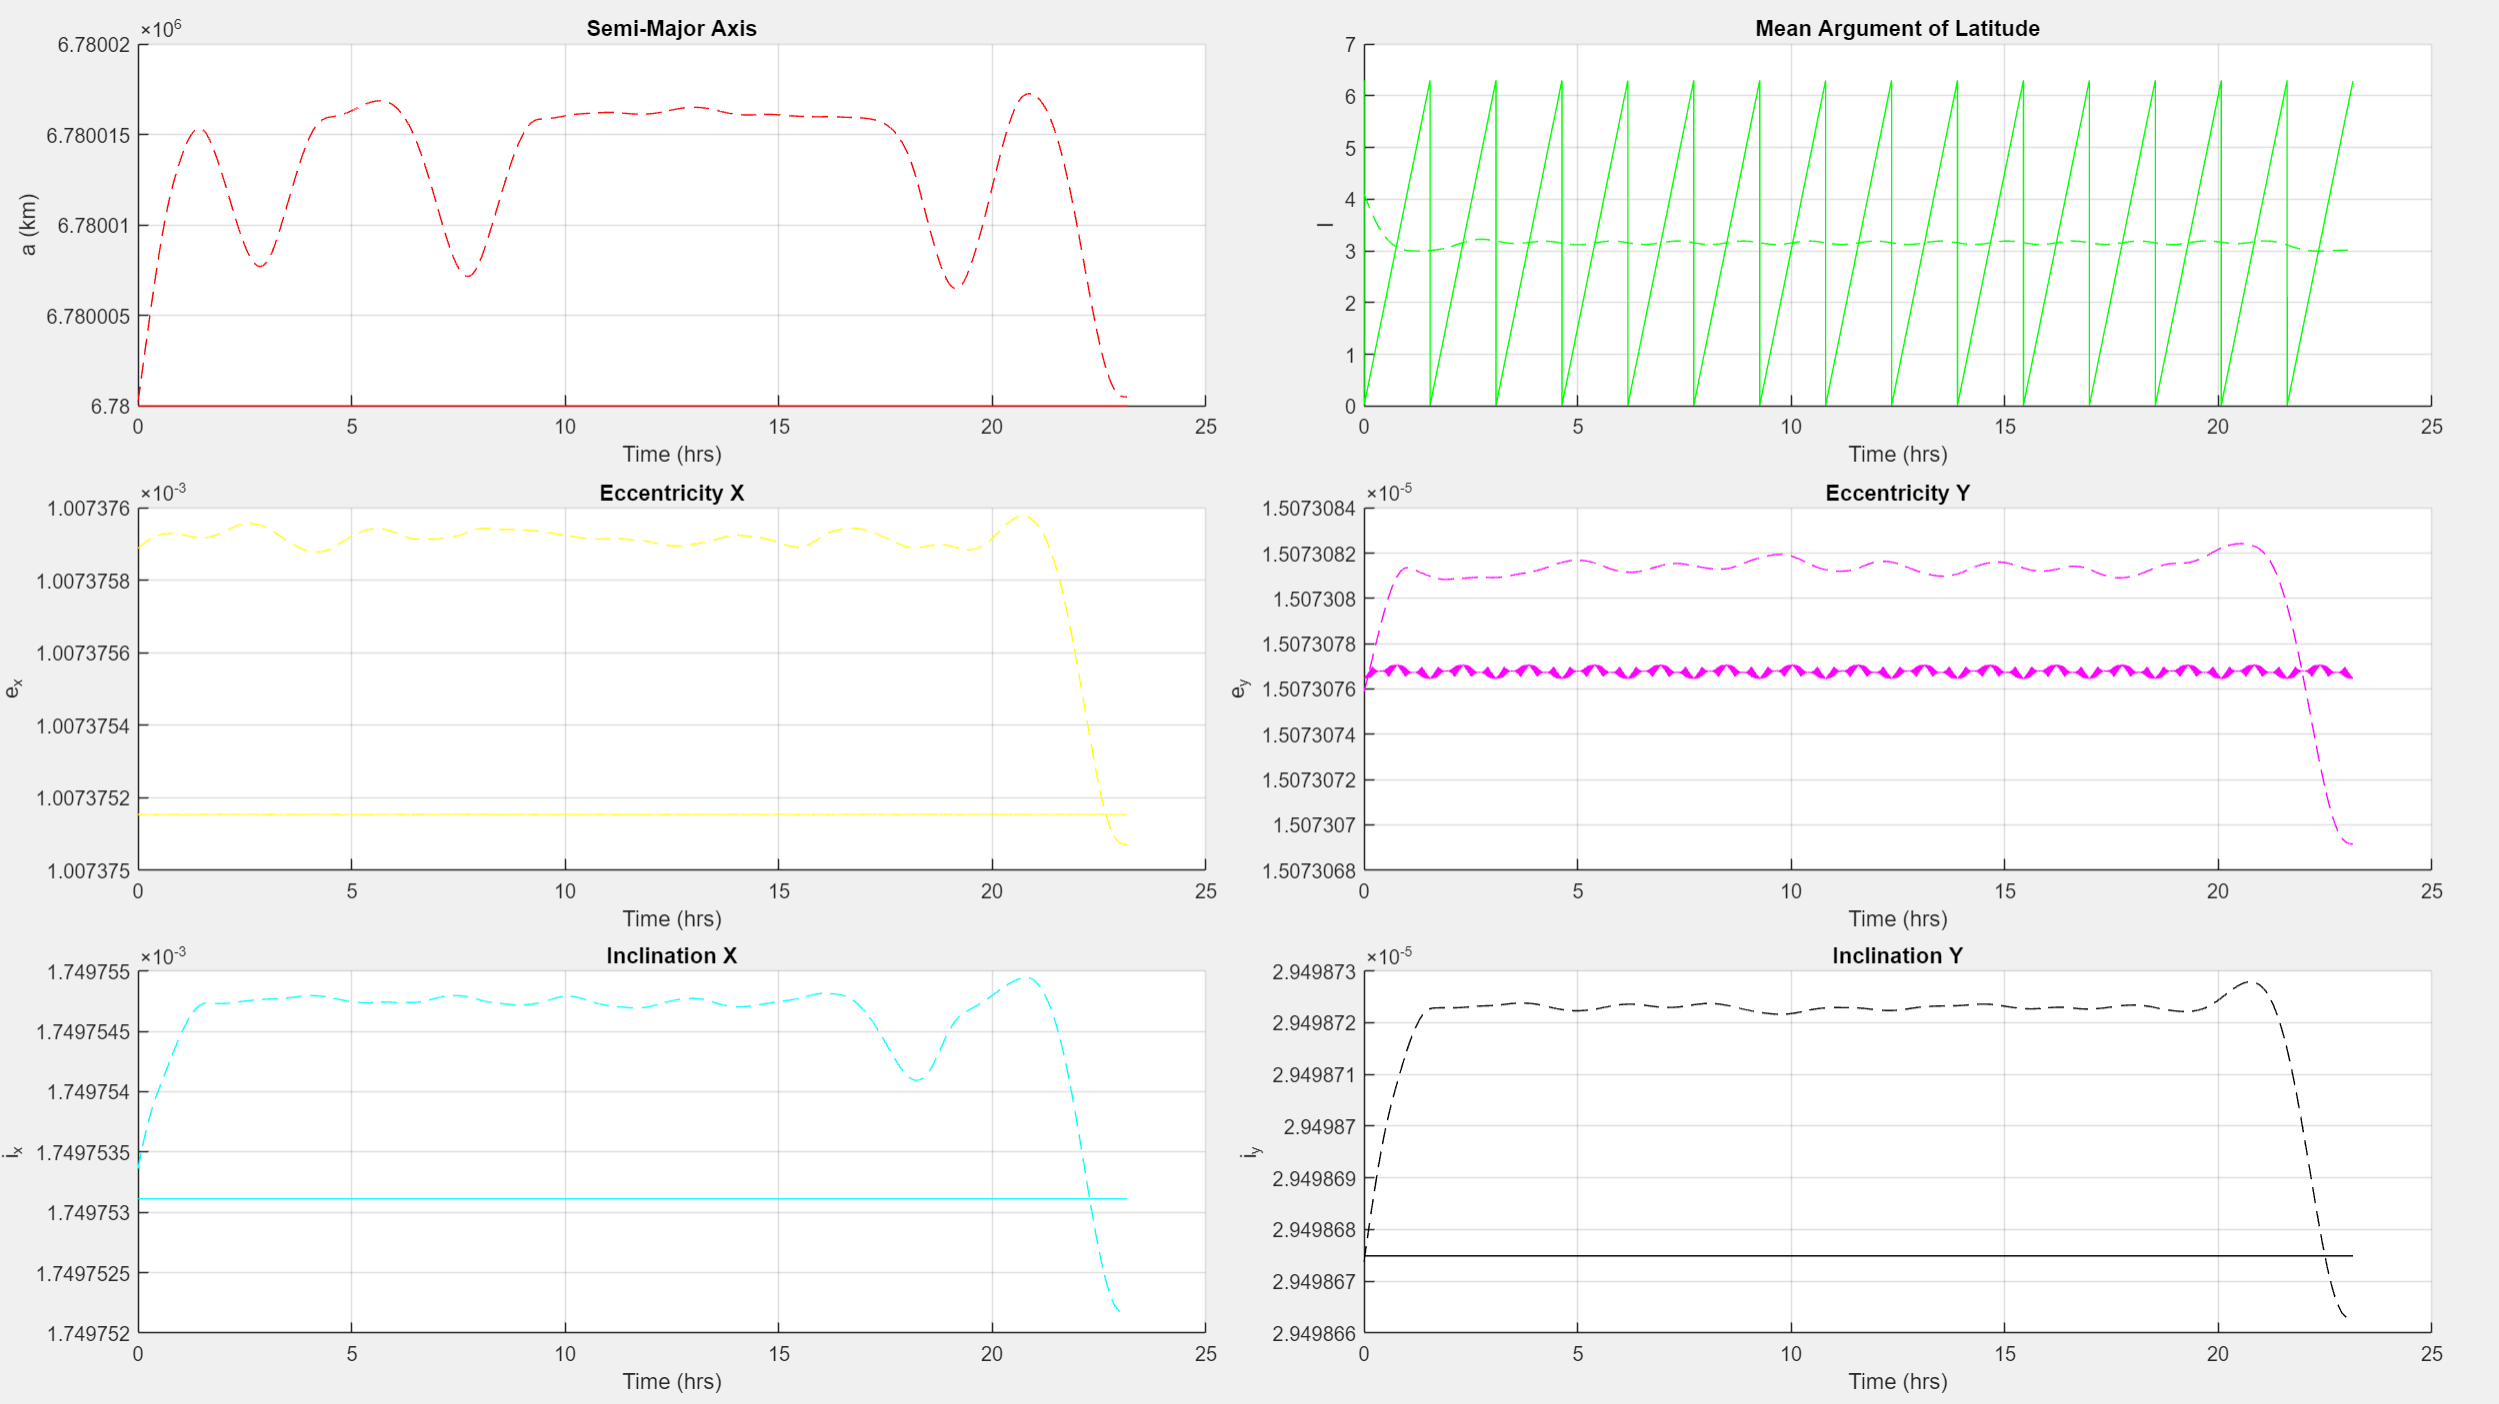
\includegraphics[width=0.7\textwidth]{PS4/Figures/case2_noJ2.png}
    \caption{Initial Conditions 2, Without J2, Quasi Nonsingular Orbital Elements}
    \label{fig:hcw_velocity}
\end{figure}
\begin{figure}[H]
    \centering
    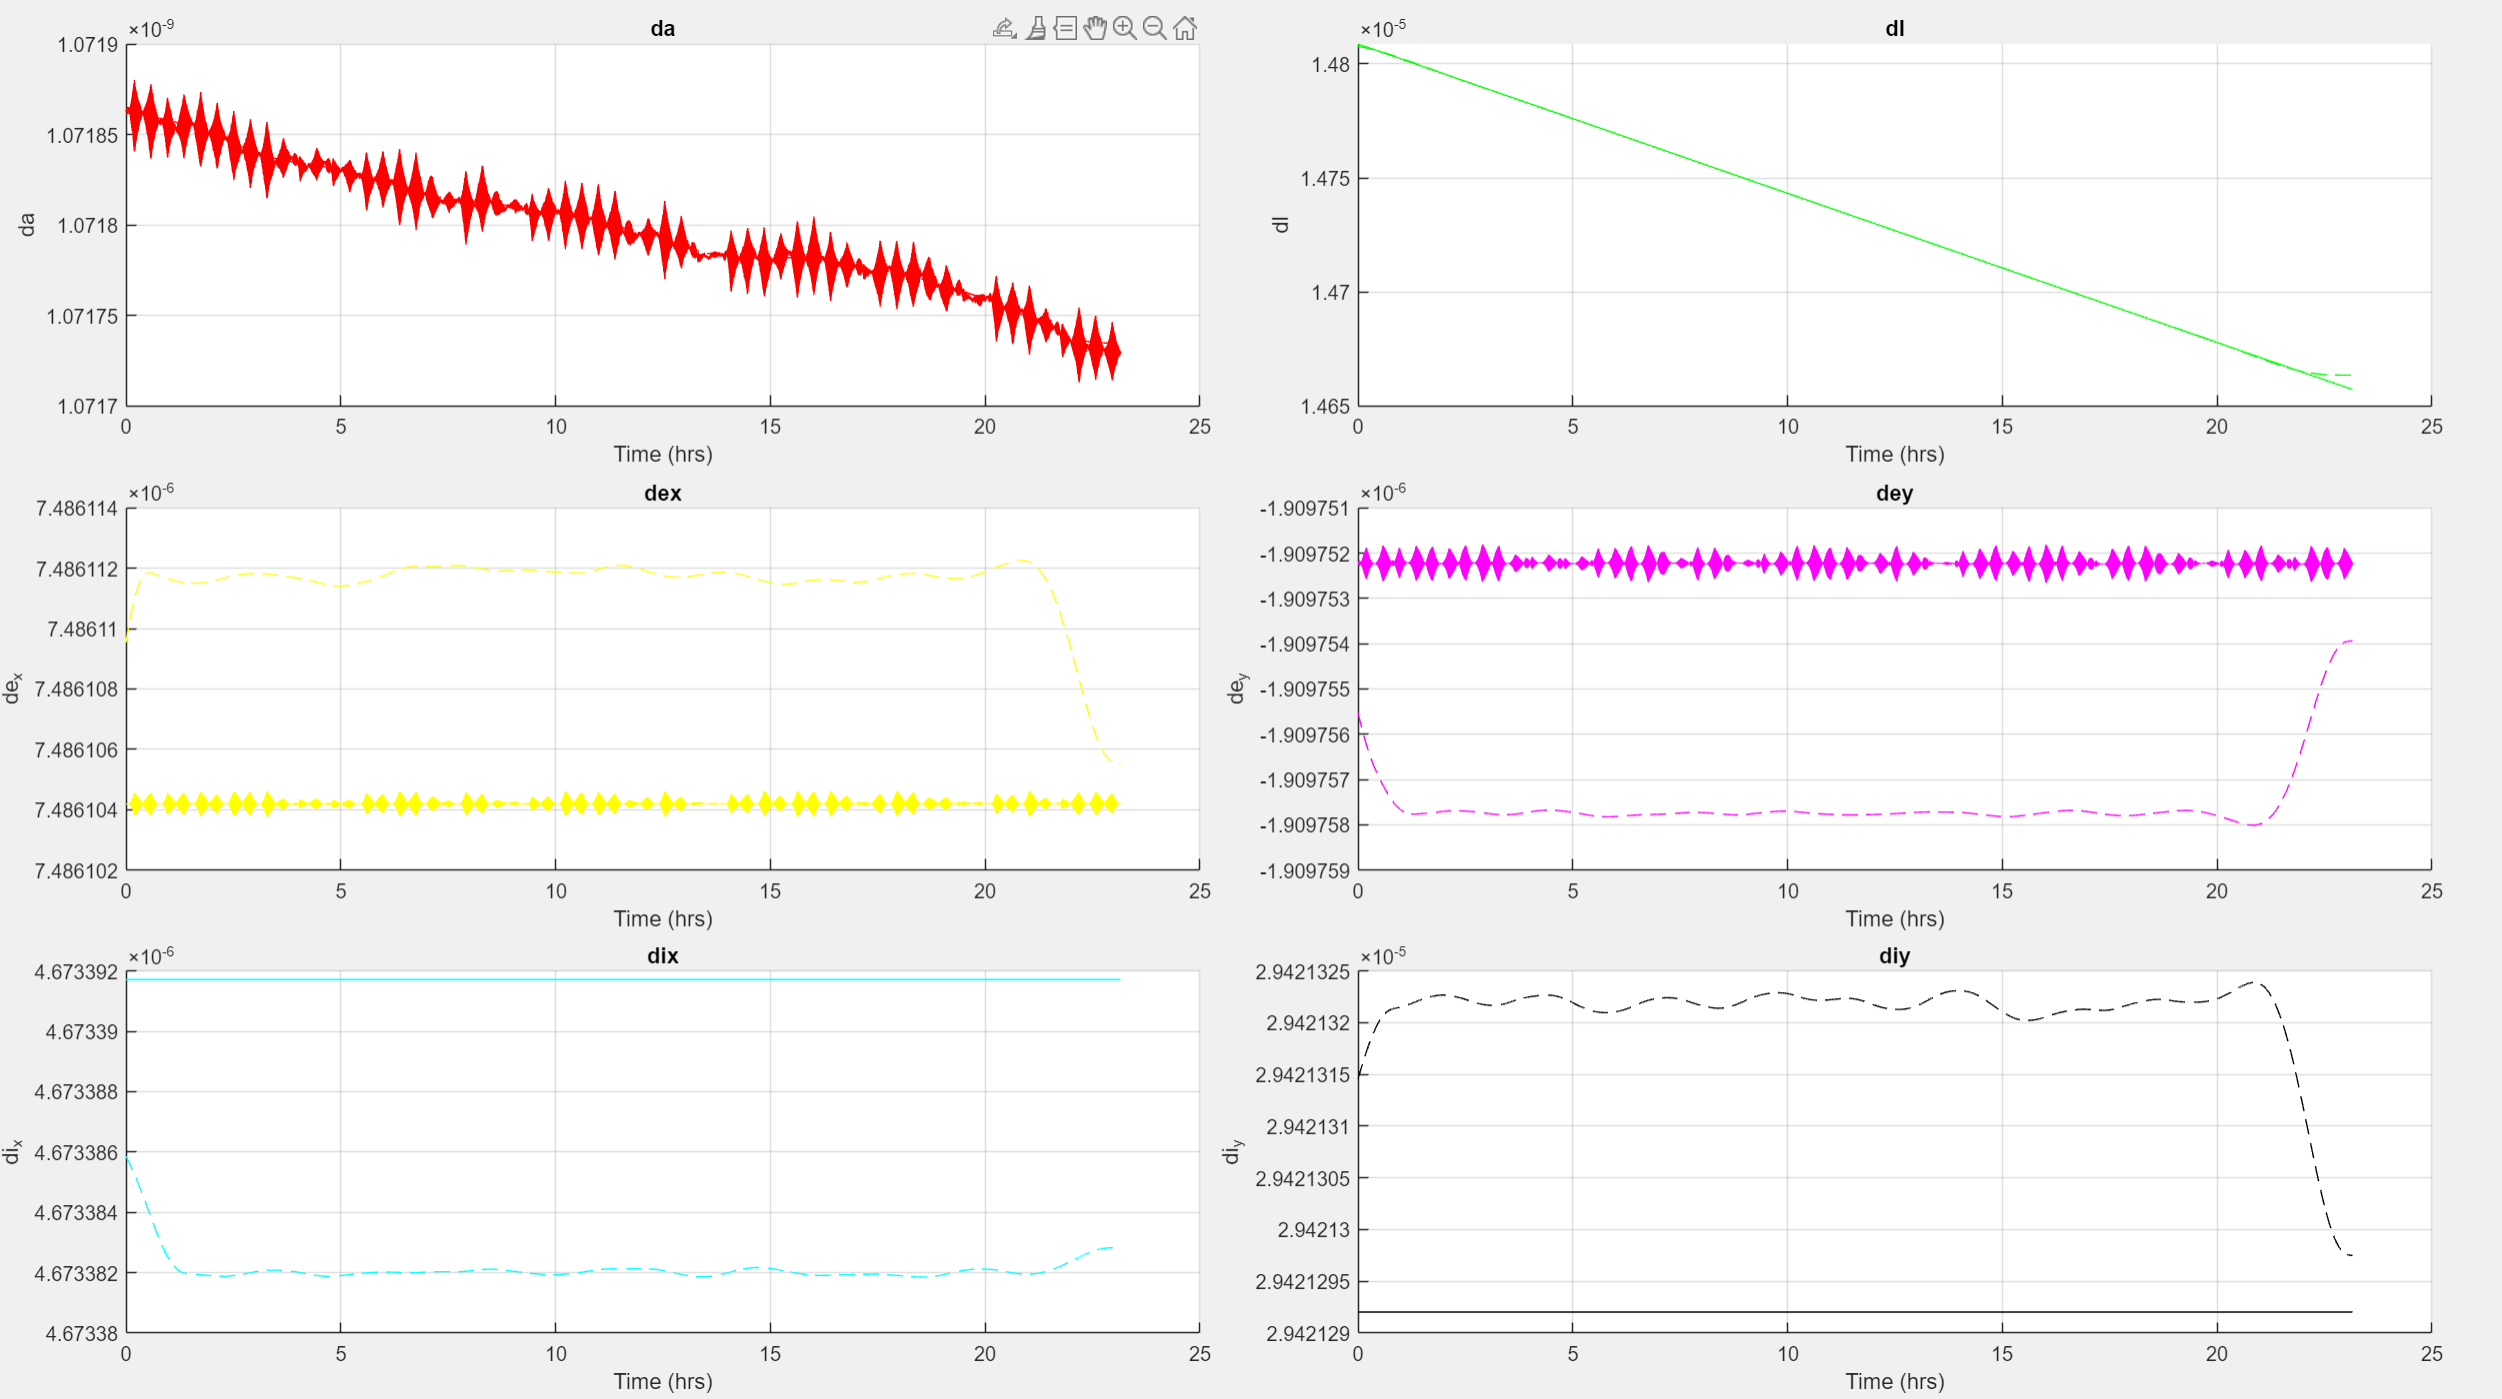
\includegraphics[width=0.7\textwidth]{PS4/Figures/case2_noJ2_2.png}
    \caption{Initial Conditions 2, Without J2, Quasi Nonsingular Relative Orbital Elements}
    \label{fig:hcw_velocity}
\end{figure}
Second part, with J2:
\begin{figure}[H]
    \centering
    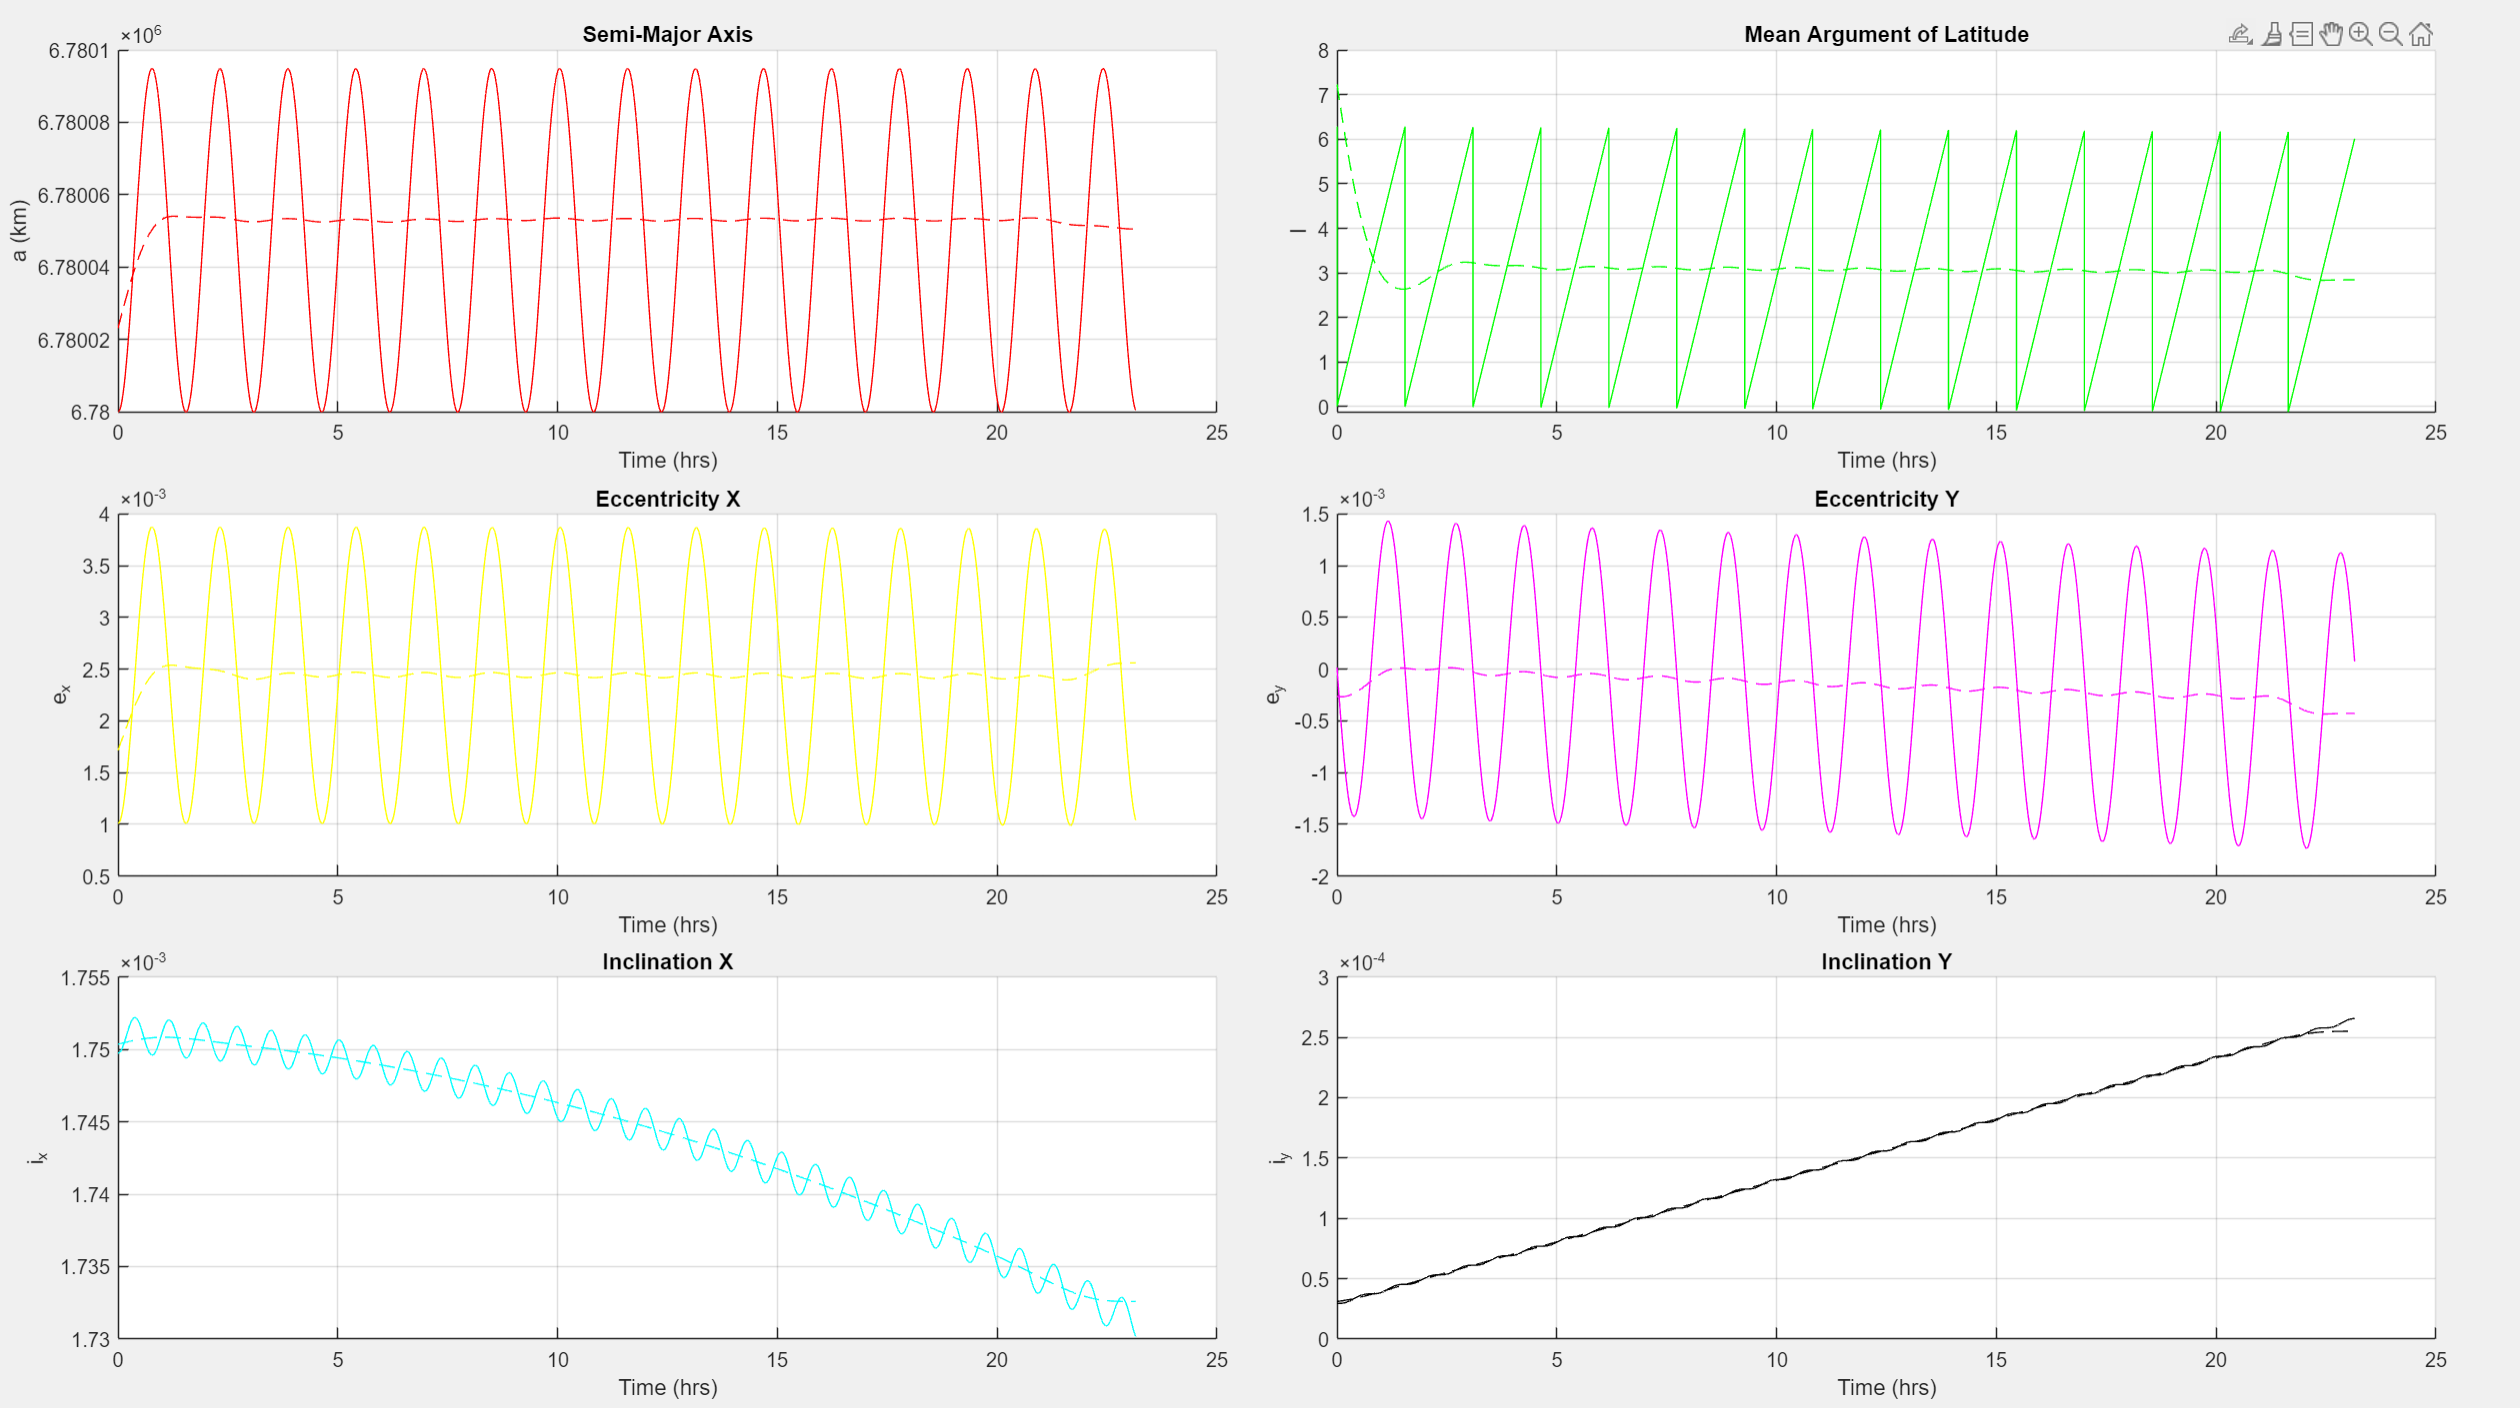
\includegraphics[width=0.7\textwidth]{PS4/Figures/case2_J2.png}
    \caption{Initial Conditions 2, with J2, Quasi Nonsingular Orbital Elements}
    \label{fig:hcw_velocity}
\end{figure}
\begin{figure}[H]
    \centering
    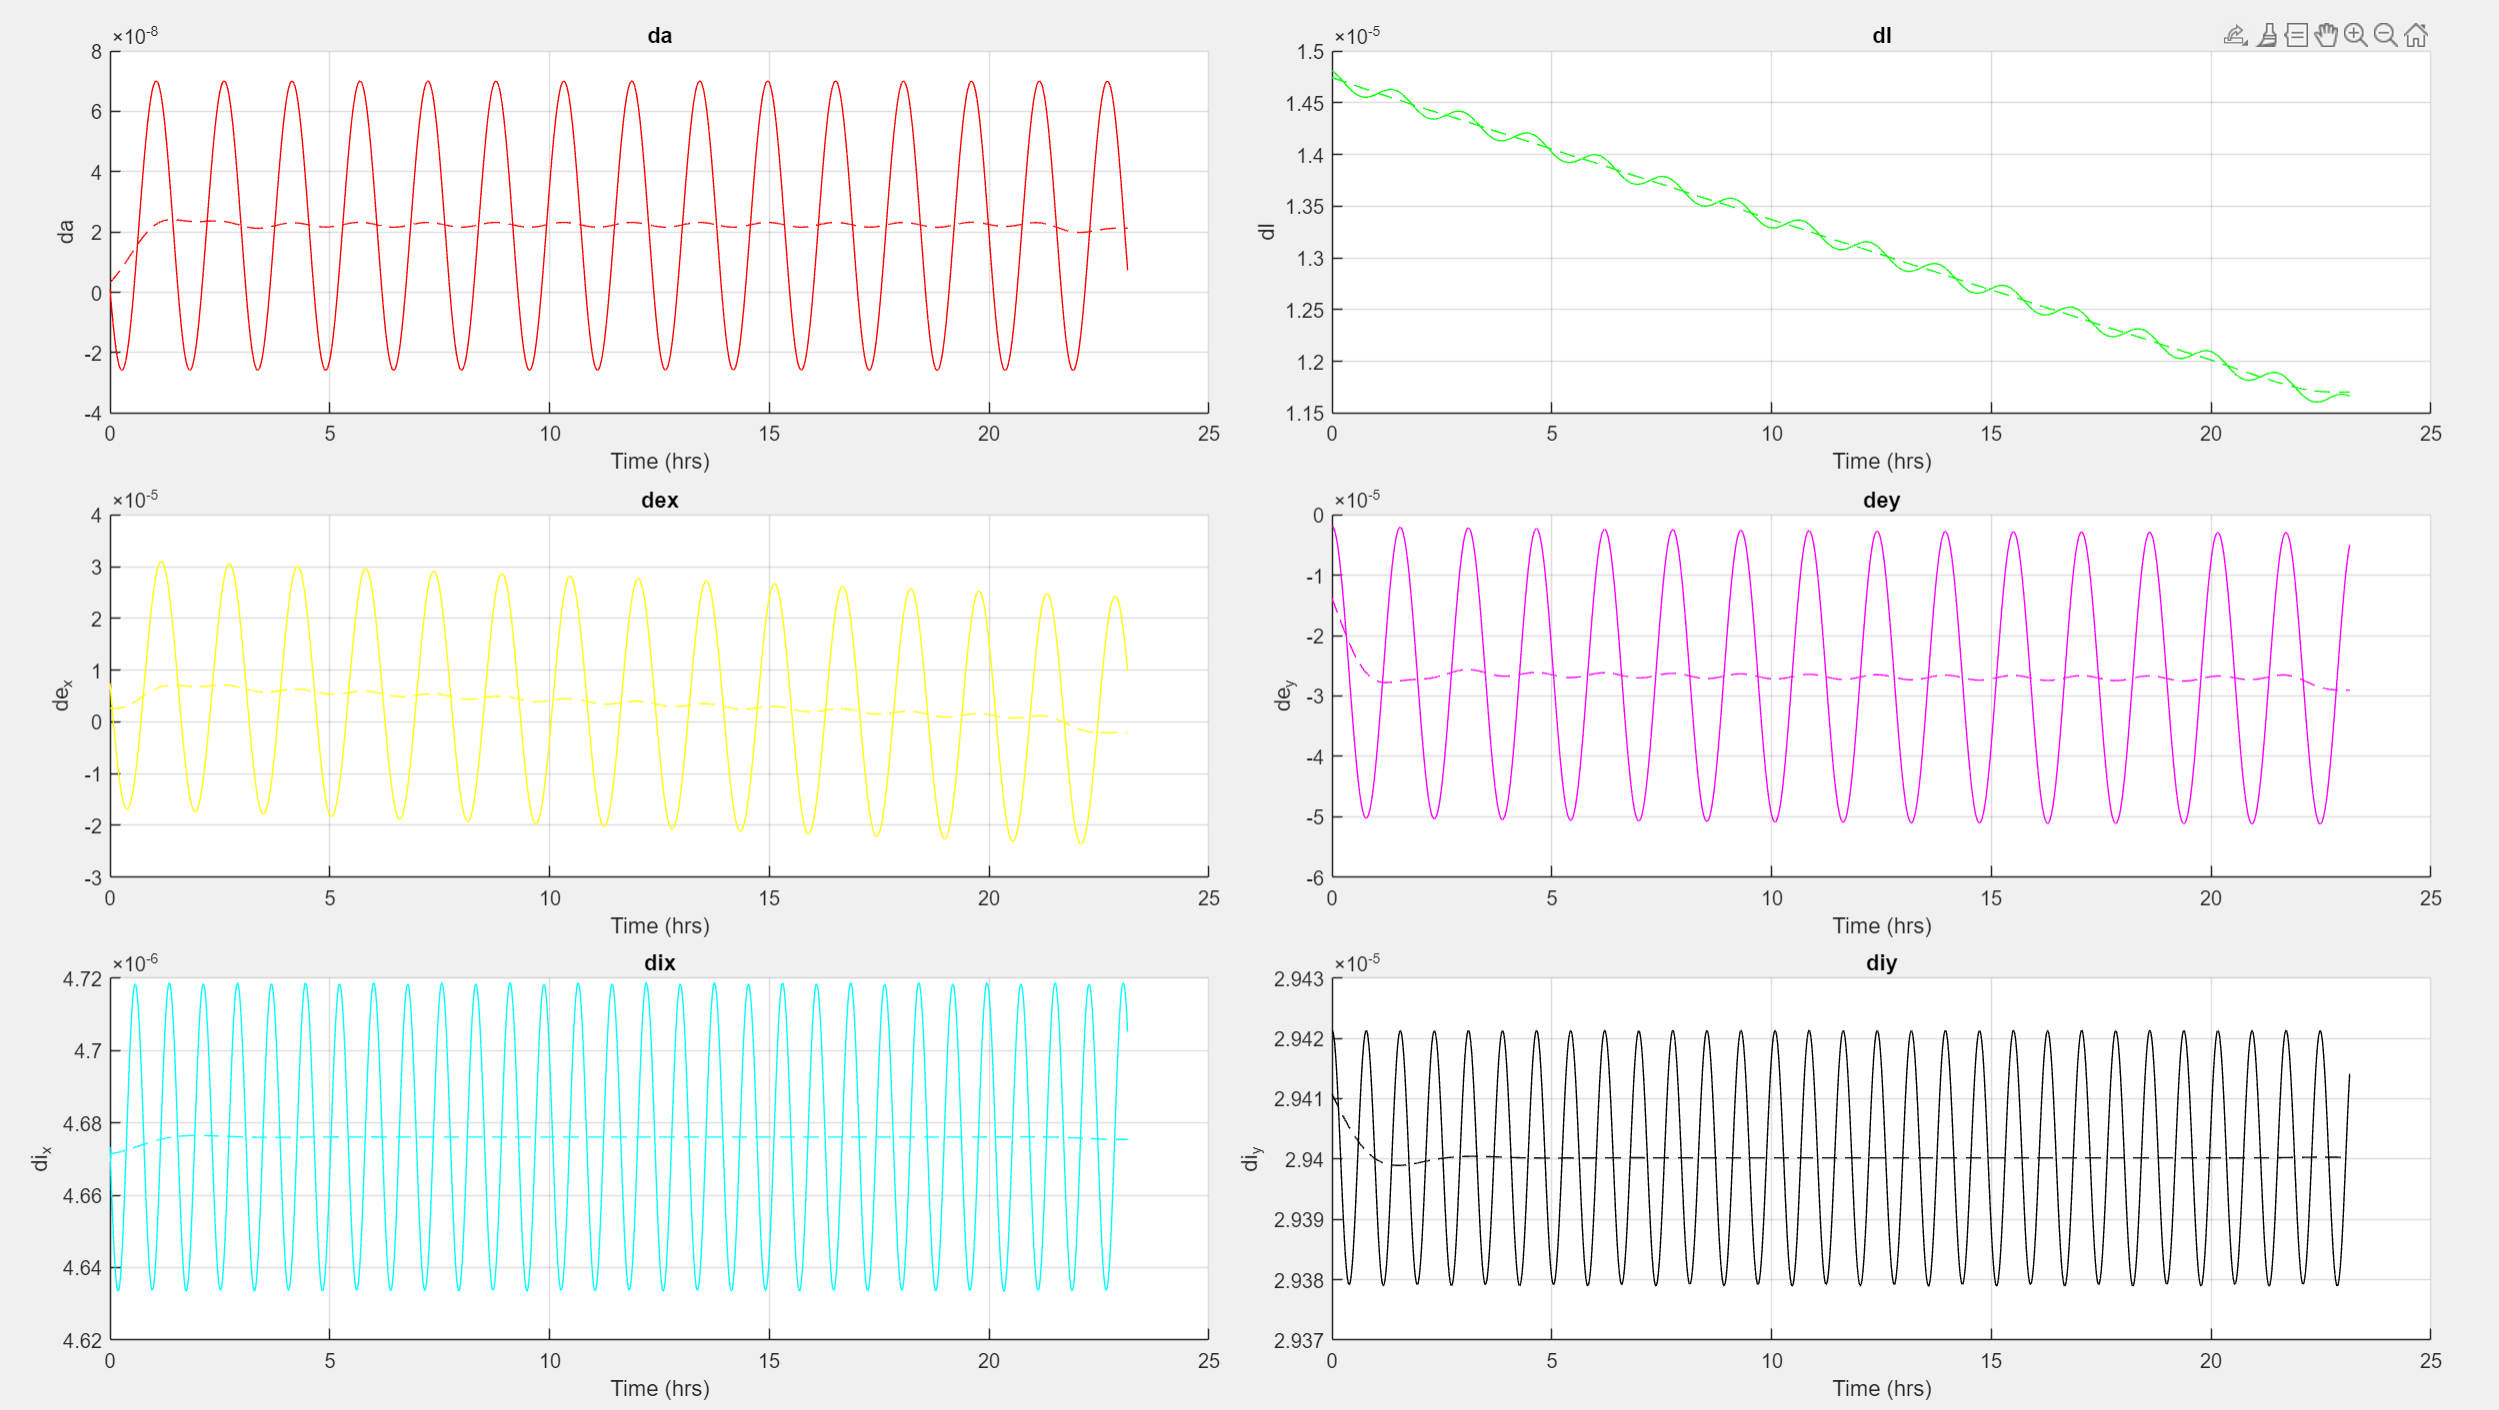
\includegraphics[width=0.7\textwidth]{PS4/Figures/case2_J2_2.png}
    \caption{Initial Conditions 2, with J2, Quasi Nonsingular Relative Orbital Elements}
    \label{fig:hcw_velocity}
\end{figure}

\subsubsection{Simulation with and without J2}
\begin{figure}[H]
    \centering
    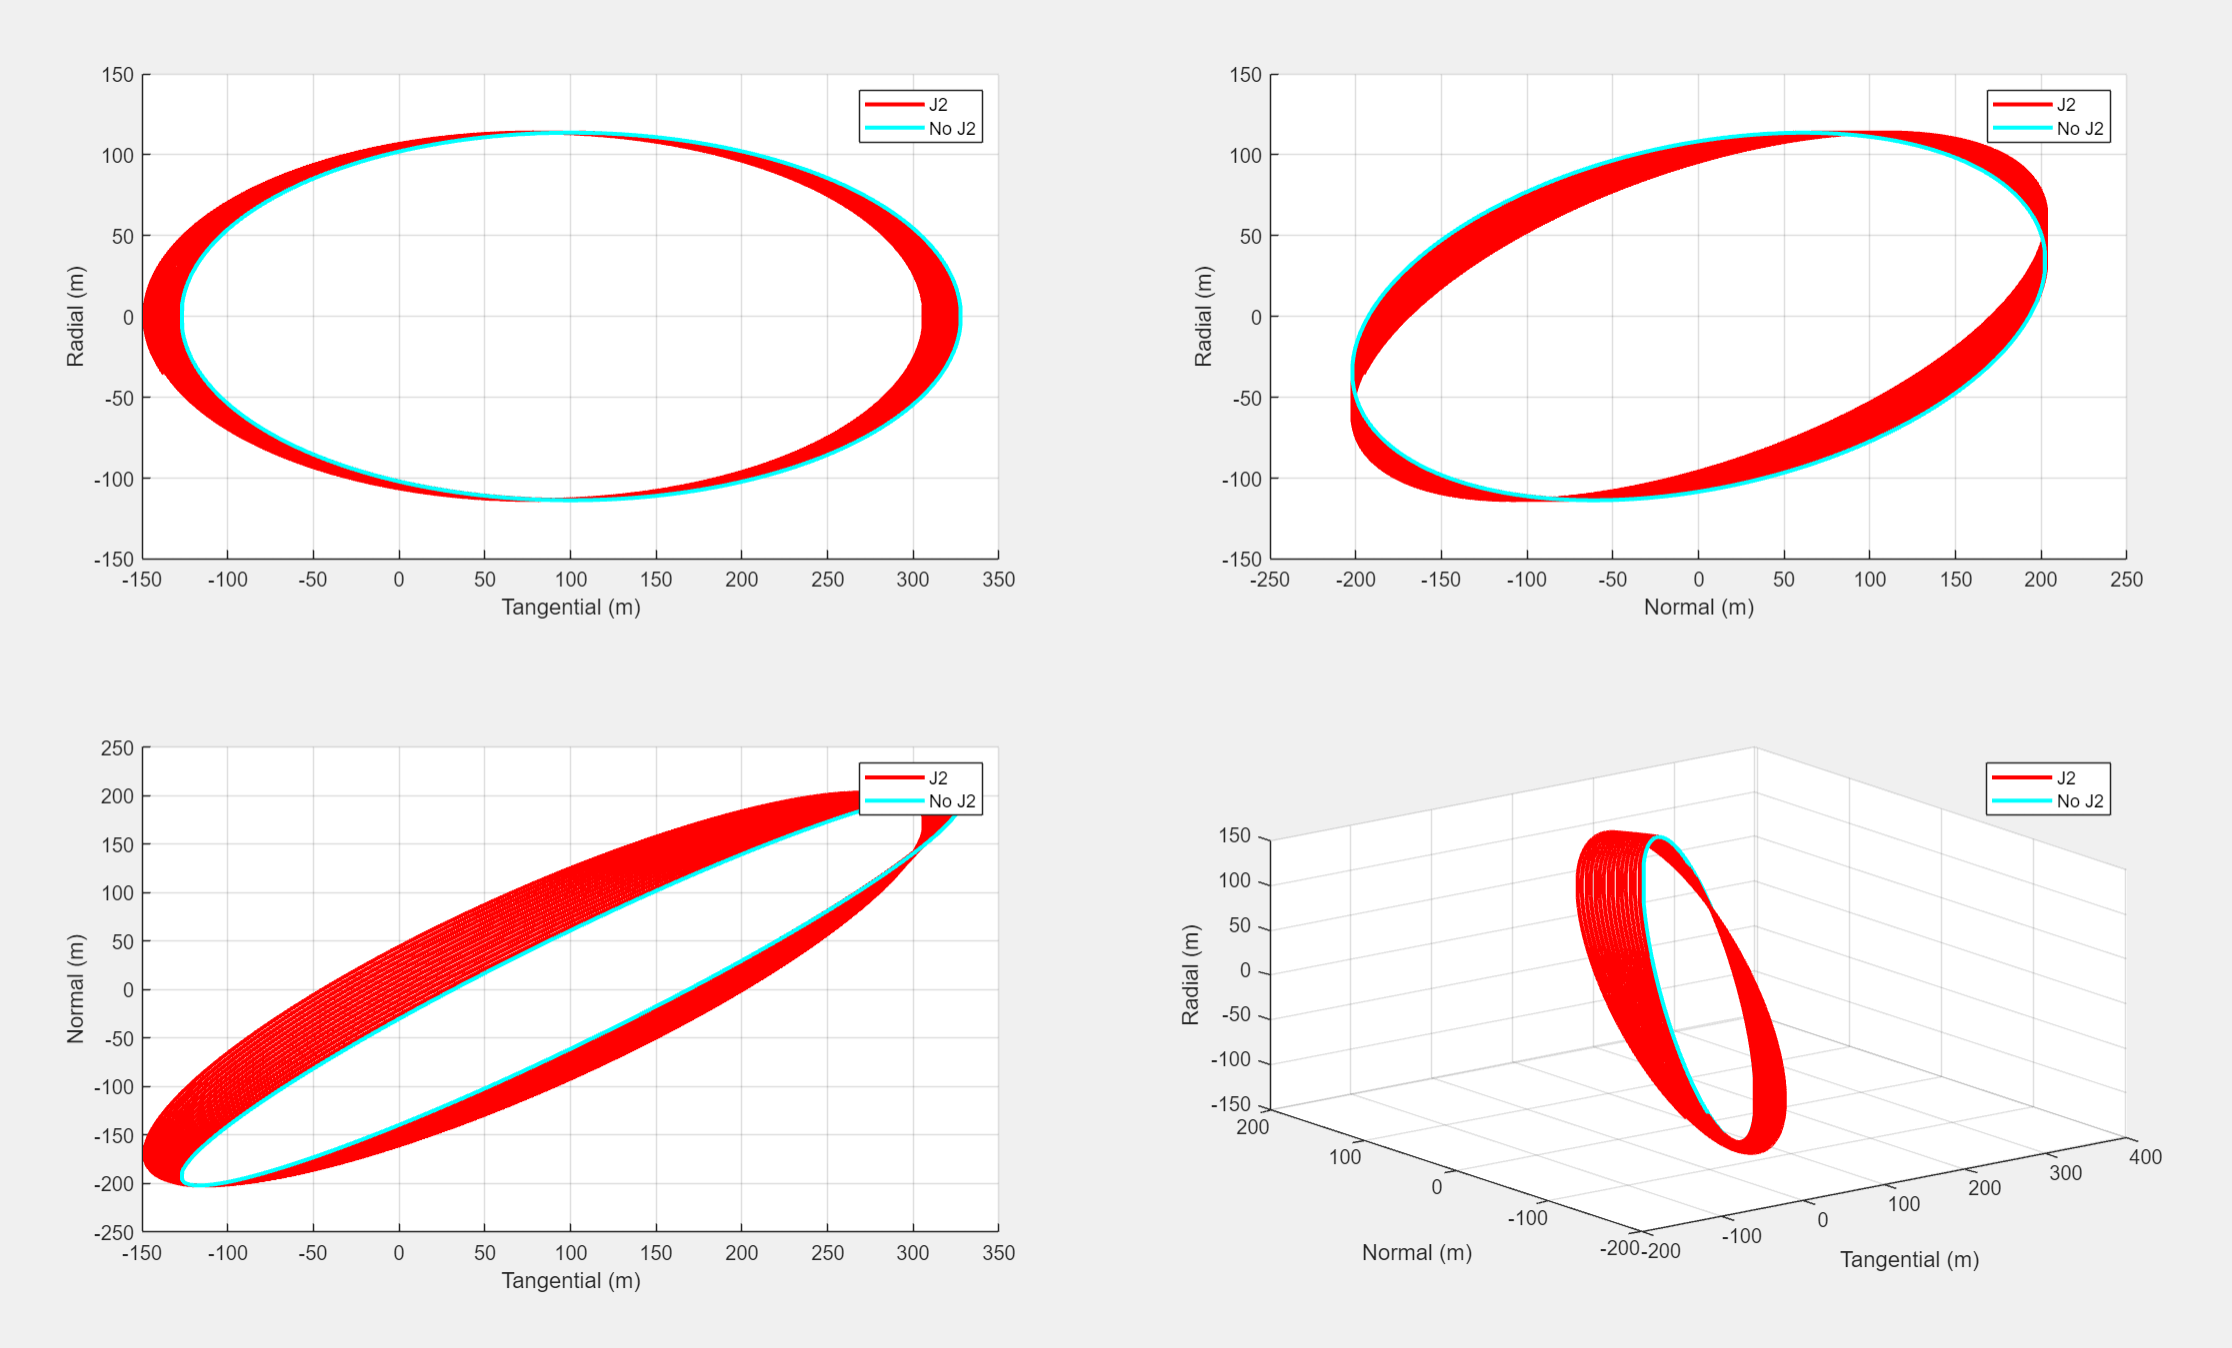
\includegraphics[width=0.7\textwidth]{PS4/Figures/rtn_position.png}
    \caption{RTN Position}
    \label{fig:hcw_velocity}
\end{figure}
\begin{figure}[H]
    \centering
    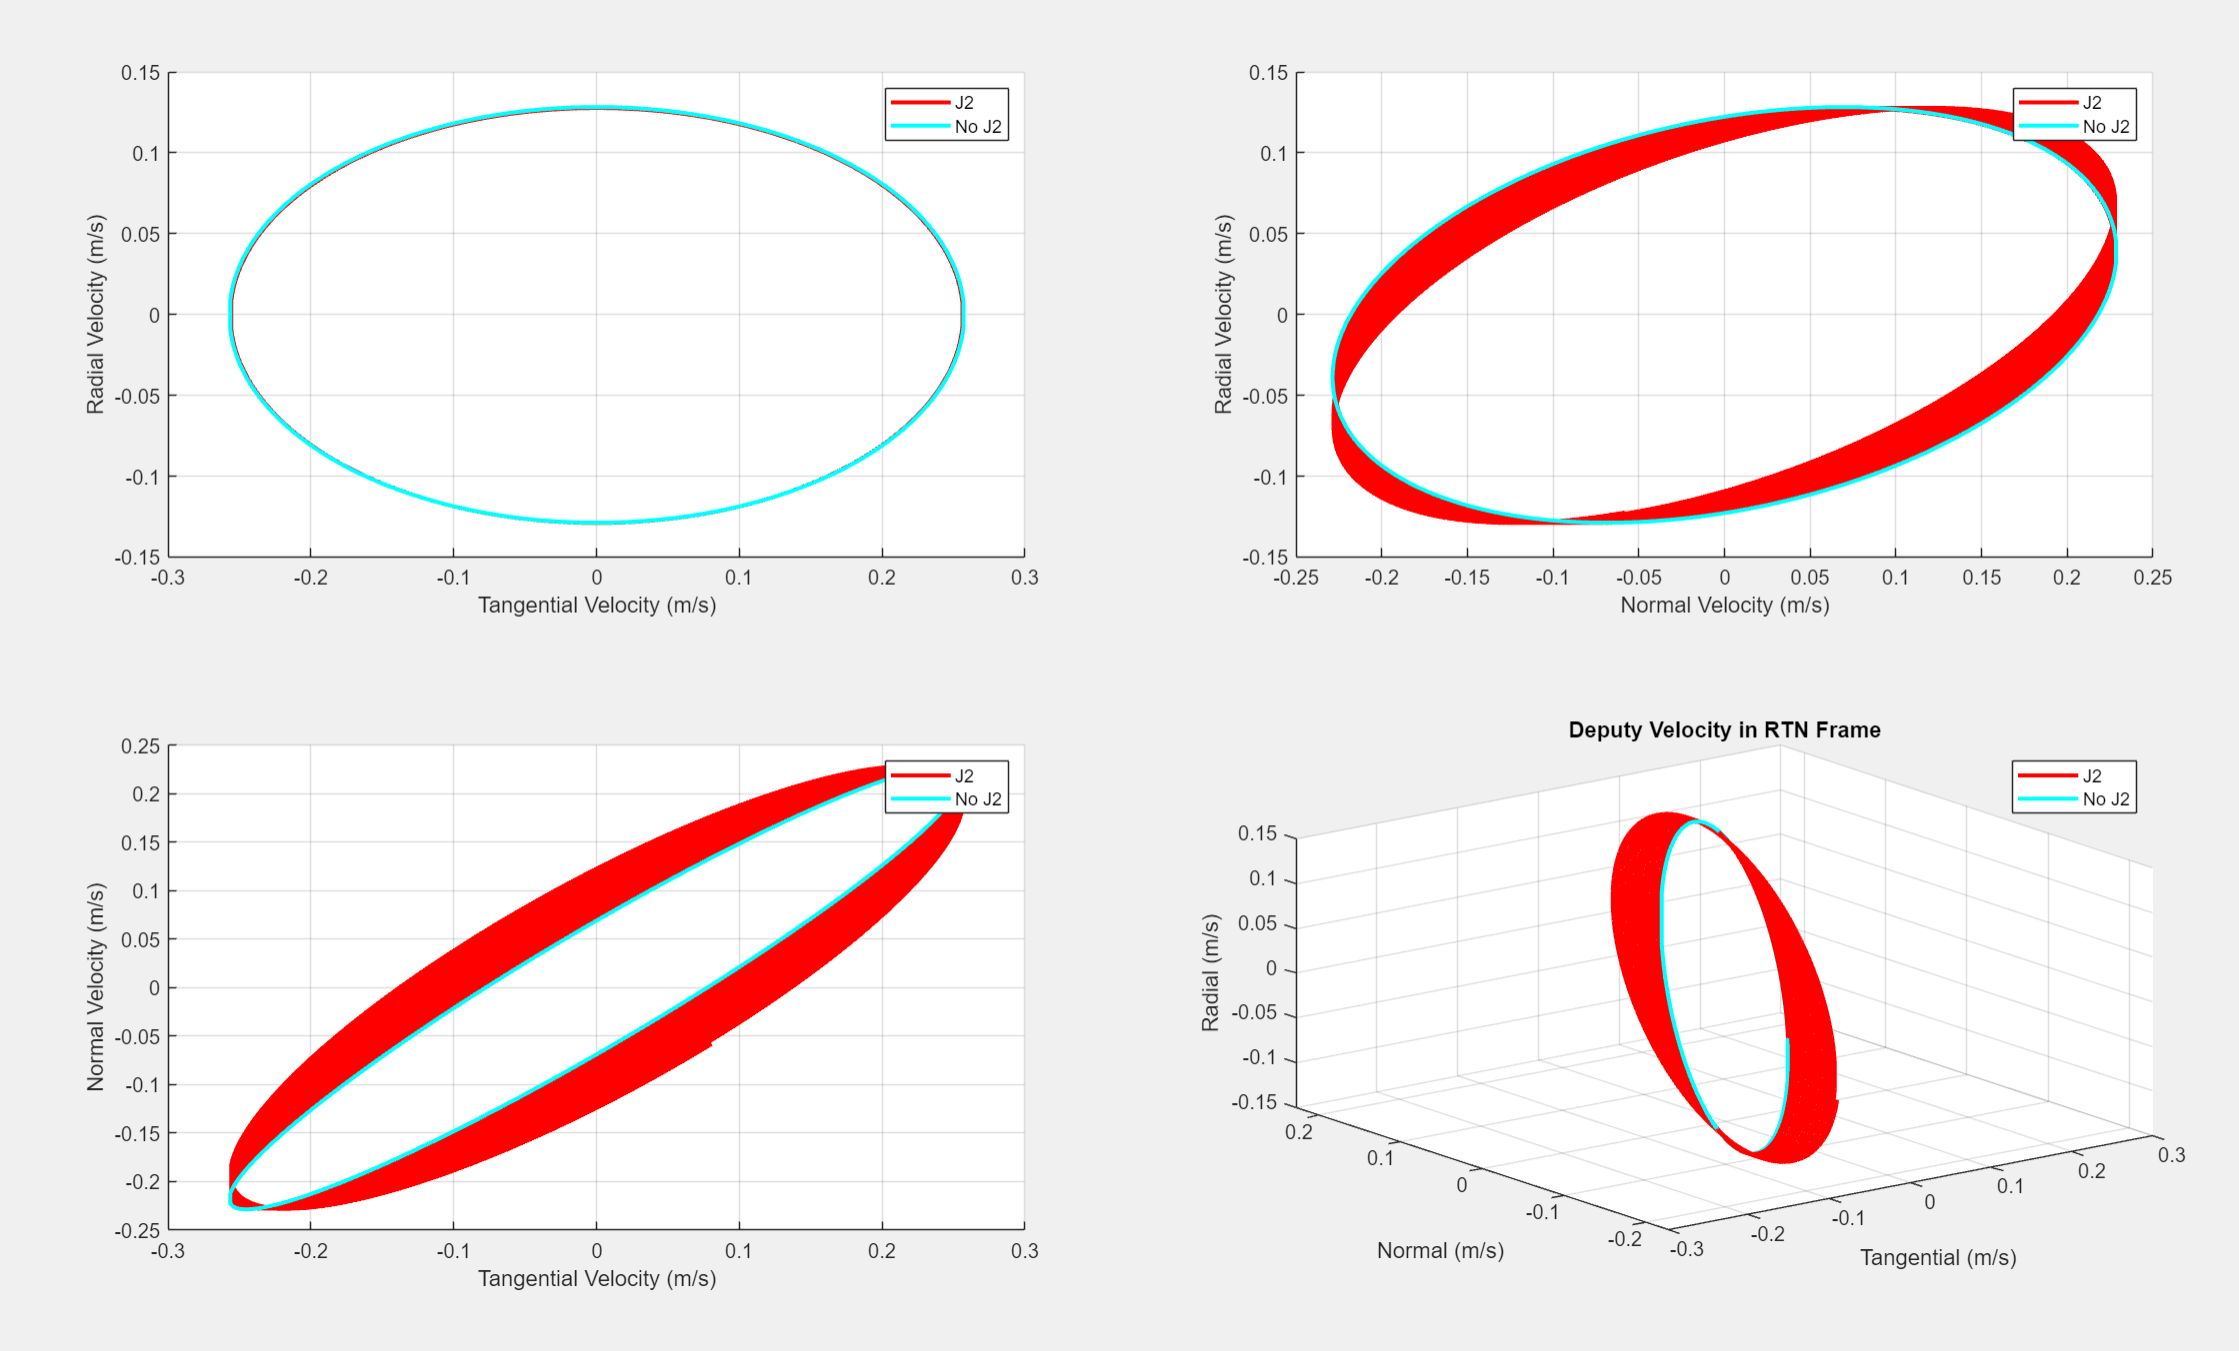
\includegraphics[width=0.7\textwidth]{PS4/Figures/rtn_velocity.png}
    \caption{RTN Velocity}
    \label{fig:hcw_velocity}
\end{figure}

\subsubsection{Planar Plots with J2 Effects}
In the following plots, the solid lines are the osculating and the dotted lines are the means.
\begin{figure}[H]
    \centering
    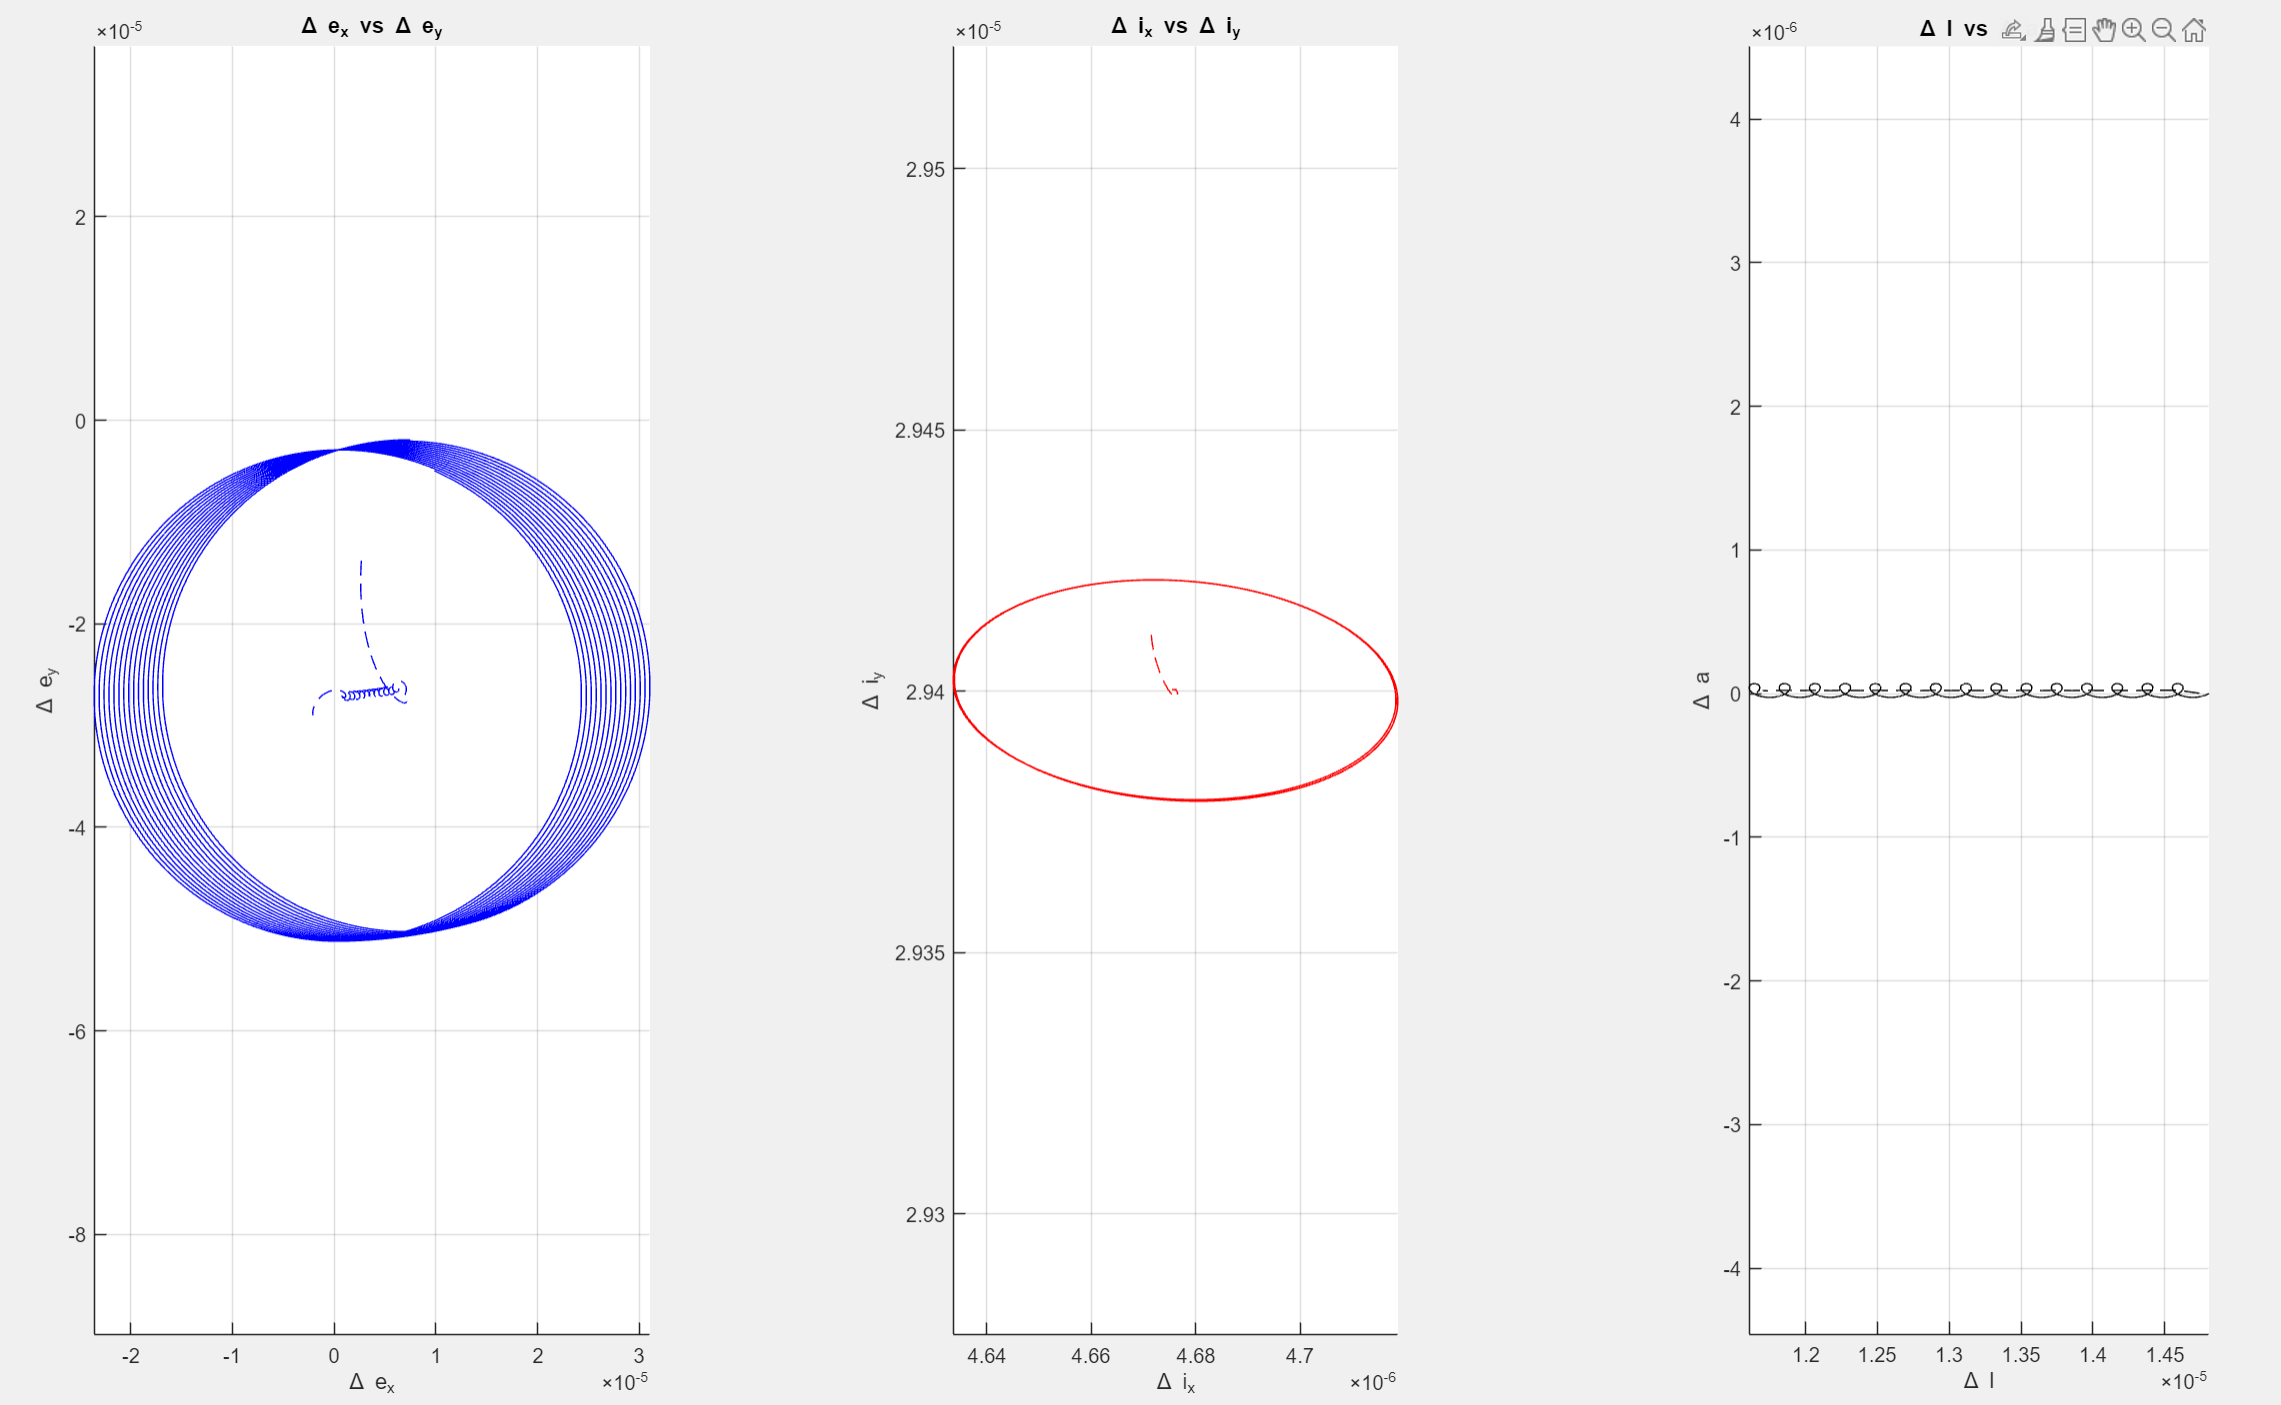
\includegraphics[width=0.7\textwidth]{PS4/Figures/problem5.png}
    \caption{Planar Plots of Roes over Time with J2 effects}
    \label{fig:hcw_velocity}
\end{figure}

\subsubsection{Drift Due to J2}
As Professor D'Amico discussed in class, one could leverage a difference in specific mechanical energy to cancel J2. If the da orbital element is approximately equal to 1000 times the differential inclination elements, the effect of J2 will negate the keplerian drift, thus rendering a stable situation. 

To do this with our initial conditions, we start with the equation $\delta \lambda' = -\frac{21}{2} \left( \gamma \sin(2i)\, \delta i_x + \frac{1}{7} \delta a \right)$. By substituting in our known inclination, a zero change rate of delta lambda, and our known inclination component in the x direction, we can obtain a delta a of 10.43m. Therefore, we must increase our semi major axis by 10.43m, which translates to a prograde burn with a delta v of 9.51 m/s. These calculations were done by using the necessary change in semi major axis and the vis a via equation. When we re-ran our simulation with these new initial conditions we saw that the secular effects were almost entirely removed.


\subsubsection{Adding STM J2 effects}

The plot below shows the comparison between numerical integration and analytical STM solution.

\begin{figure}[H]
    \centering
    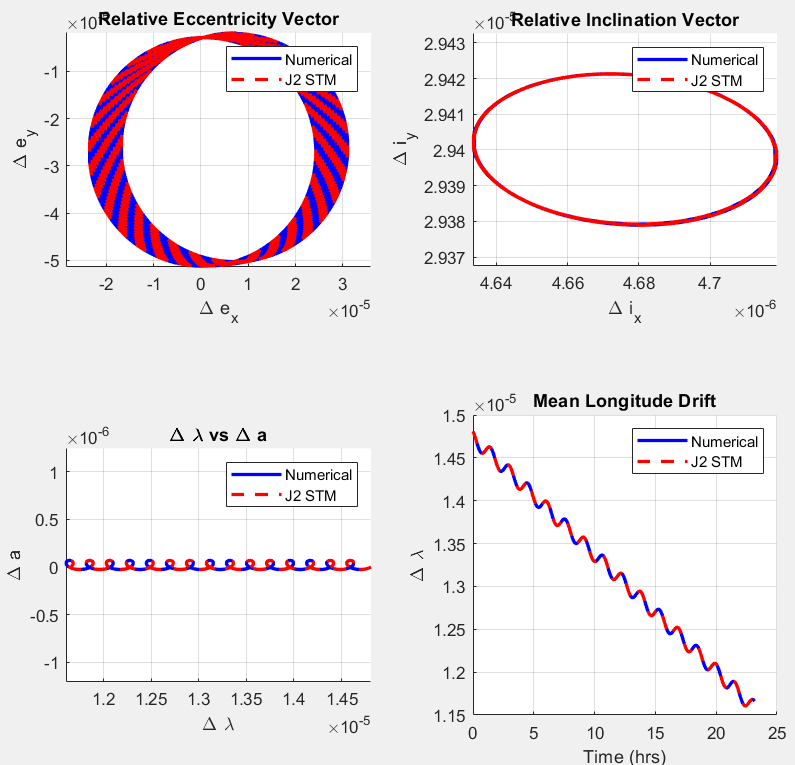
\includegraphics[width=0.7\textwidth]{PS4/Figures/ROE_STM_Comparison.png}
    \caption{STM J2 comparison.}
    \label{fig:stm_comparison}
\end{figure}